\documentclass[12pt]{article}
\usepackage[utf8]{inputenc}
\usepackage[T1]{fontenc}
\usepackage{mathptmx}
\usepackage{geometry}
\usepackage{mathtools}
\usepackage[english]{babel}
\usepackage{graphicx}
\usepackage[figurename=Gambar]{caption}
\usepackage{hyperref}
\usepackage{minted}
\usepackage{setspace}
\usepackage{color}
\usepackage[explicit]{titlesec}
\usepackage{tocloft}
\usepackage{titletoc}
\usepackage{indentfirst}
\usepackage{caption}
\usepackage{subcaption}
\usepackage{amsmath} 
\usepackage{pdfpages}

%\color{white}
%\pagecolor{black}

\hypersetup{colorlinks,
	citecolor=black,
	filecolor=black,
	linkcolor=black,
	urlcolor=black
}

\geometry{
	a4paper,
	left=30mm,
	right=25mm,
	top=15mm,
	bottom=15mm,
}

\date{}

%=============================================================================
% Modified Items

\providecommand{\keywordid}[1]{\textit{Kata Kunci: } #1}
\providecommand{\keyworden}[1]{\textit{Keywords: } #1}

\titleformat{\section}{}{}{0pt}{}
\titleformat{\subsubsection}{\small \bfseries}{\thesubsection}{0pt}{}

\renewcommand{\cftsecleader}{\cftdotfill{\cftdotsep}}
\renewcommand{\cftsubsecleader}{\cftdotfill{\cftdotsep}}

\makeatletter
\let\latexl@section\l@section
\def\l@section#1#2{\begingroup\let\numberline\@gobble\latexl@section{#1}{#2}\endgroup}
\makeatother

\addto\captionsenglish{\renewcommand{\contentsname}{}}
\addto\captionsenglish{\renewcommand{\listfigurename}{}}

\renewcommand{\cftsecfont}{\normalfont}
\renewcommand{\cftsecpagefont}{\normalfont}

\renewcommand{\thefigure}{\arabic{section}.\arabic{figure}}

\hyphenation{mau-pun berdasar-kan}

%=============================================================================
% Document Part

\begin{document}

\addtocounter{section}{-6}
\onehalfspacing

%=============================================================================

% Cover
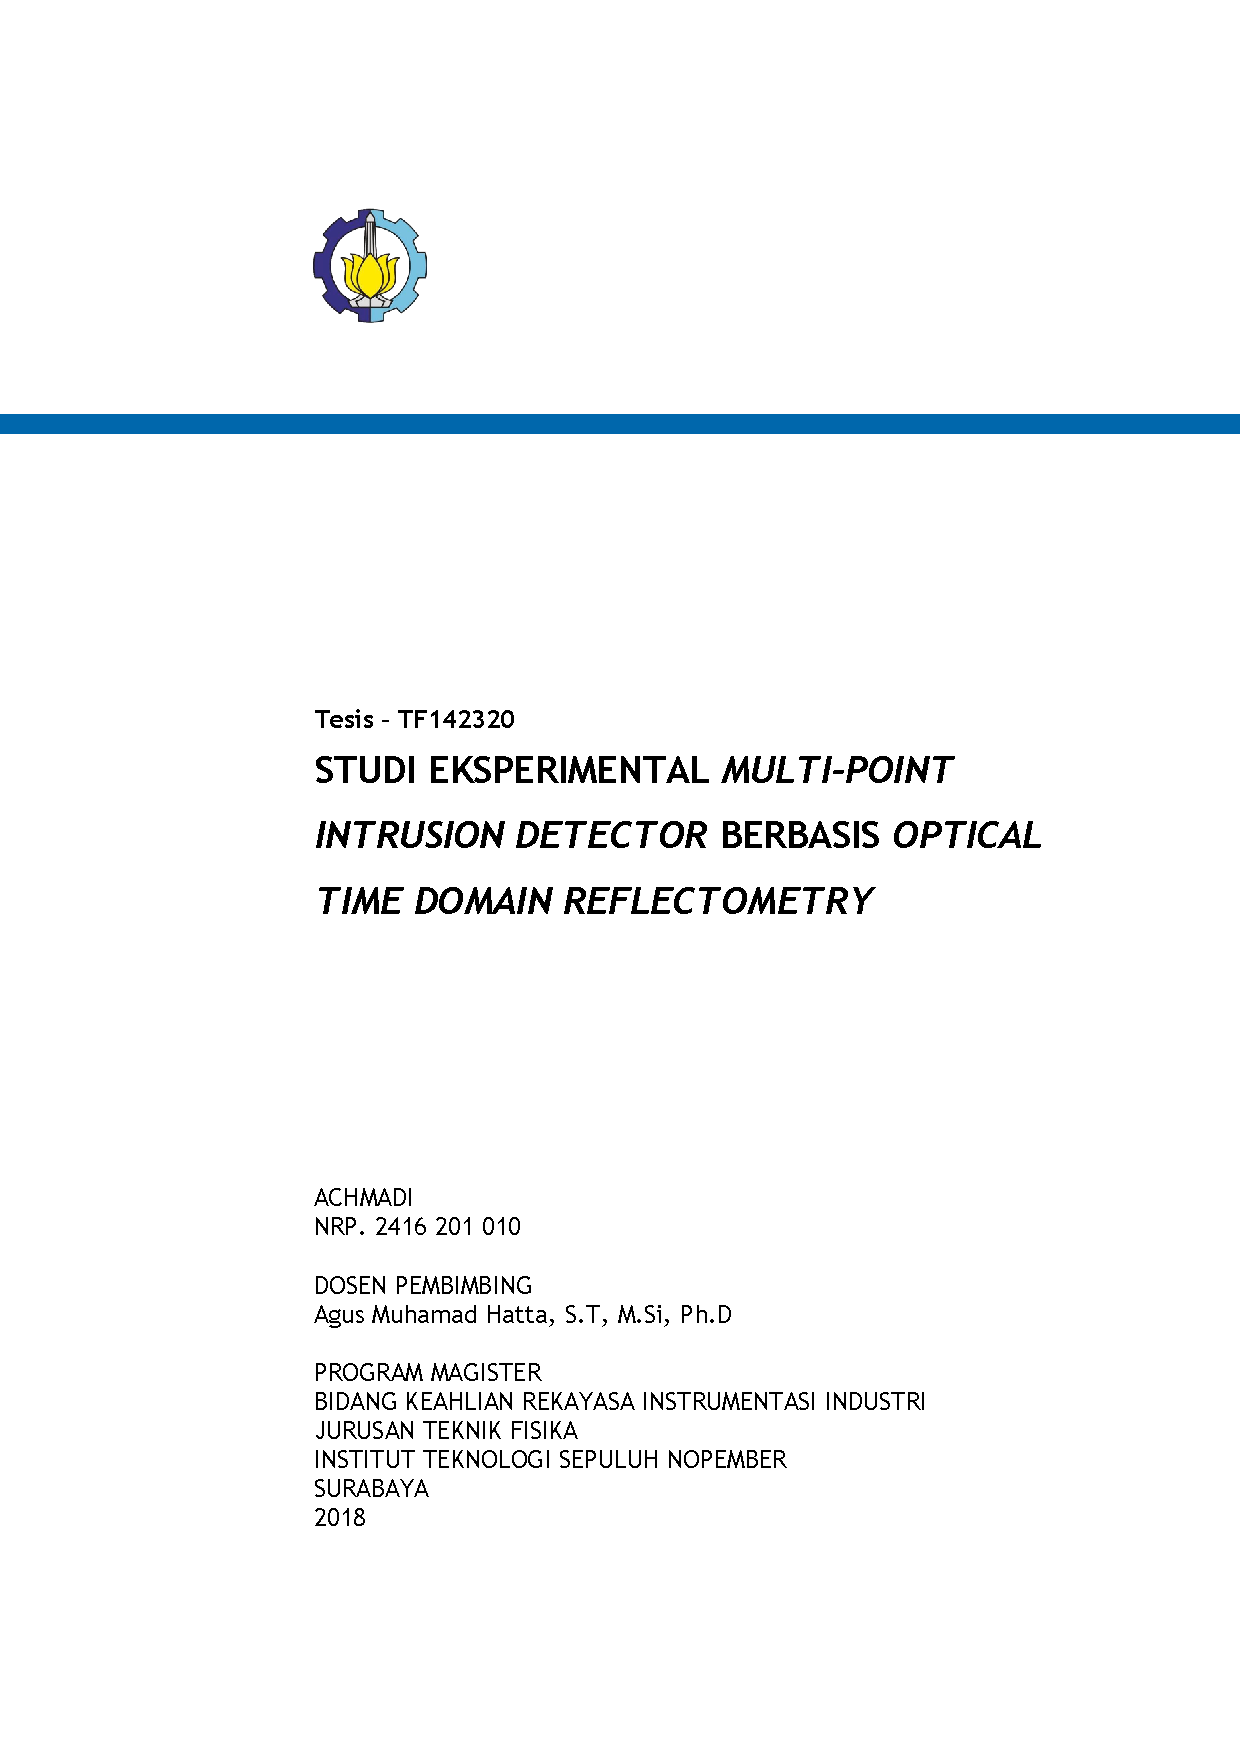
\includepdf[pages=-]{images/cover.pdf}

%=============================================================================

%\newpage
%\thispagestyle{plain}
%\mbox{}

%=============================================================================
% Abstrak Indonesia
	
	\pagenumbering{roman} 
	\setcounter{page}{3}

	\section{Abstrak}
	
	\begin{center}
		\large{\textbf{STUDI EKSPERIMENTAL \textit{MULTI-POINT INTRUSION DETECTOR} BERBASIS OPTICAL TIME DOMAIN REFLECTOMETRY}}
	\end{center}

	\vspace{10pt}
	
	\begin{flushleft}
		Nama Mahasiswa : Achmadi \\
		NRP \hspace{62pt}: 24 16 201 010 \\
		Pembimbing \hspace{24pt}: Agus Muhamad Hatta, S.T, M.Si, Ph.D \\
	\end{flushleft}
	
	\vspace{10pt}

	\renewcommand{\abstractname}{ABSTRAK}
	\begin{abstract}
		Penyusup (\textit{intruder/attacker}) merupakan sebuah aktifitas yang tidak bisa dianggap untuk tidak mungkin terjadi apabila berkaitan dengan bangunan, area (perimeter), maupun objek lain dimana memiliki suatu nilai baik militer, ekonomi, maupun industri. 
		Tindak penyusupan memiliki similaritas dengan tindak pencurian dan menjadi awal dari tindak kriminal yang lebih jauh.
		Tindak penyusupan melalui proses melewati sistem pengawasan atau penjagaan.
		Untuk pencegahannya, maka sistem deteksi penyusup telah menjadi bagian penting dalam banyak sistem keamanan.
		Dibutuhkan sistem deteksi yang akurat dan respon yang cepat. Serat optik telah dikenal mampu menjadi transmisi data maupun sebagai sensor.
		Serat optik dapat digunakan sebagai distributed sensor yang mampu menggantikan banyak sensor tipe titik.
		OTDR telah dikenal sebagai salah satu metode karakteriasi serat optik.
		Melalui OTDR akan didapatkan events yang terjadi pada serat optik secara \textit{real-time}.
		Hasil \textit{trace} OTDR dapat digunakan untuk deteksi penyusup.
		Penelitian ini bertujuan untuk merancang sistem deteksi penyusup menggunakan serat optik dan OTDR yang mampu menemukan penyusup dalam multi-point.
		Dalam penelitian ini diusulkan sebuah studi eksperimental untuk mendapatkan rancang bangun sistem sensor terdistribusi berbasis serat optik dan OTDR untuk deteksi penyusup.
		Studi eksperimental disini divariasikan baik konfigurasi serat optik itu sendiri dan juga divariasikan bentuk distribusi sensor.
		Untuk mendapatkan hasil trace maka digunakan modul Mini-OTDR Anritsu MU909015C, sedangkan untuk eksperimen akan dibangun konstruksi pagar yang akan menjadi tempat instalasi sensor.
		Sebagai pengganti tindak intrusi maka diberikan gaya tekan kepada sensor dengan nilai dan jumlah yang telah ditentukan.
		Luaran yang diharapkan dari penelitian ini adalah hasil rancang bangun sensor instrusi terdistribusi dan rancang bangun algoritma untuk mendapatkan posisi multi-point dari tindak intrusi.   
	\end{abstract}

	\keywordid{Serat optik, OTDR, deteksi penyusup, trace, events, sensor terdistribusi}

%=============================================================================

\newpage
\thispagestyle{plain}
\mbox{}
	
%=============================================================================
% Abstrak English
	\newpage
	
	\section{Abstract}
	
	\begin{center}
		\large{\textbf{EXPERIMENTAL STUDY OF MULTI-POINT INTRUSION DETECTOR BASED ON OPTICAL TIME DOMAIN REFLECTOMETRY}}
	\end{center}
	
	\vspace{10pt}
	
	\begin{flushleft}
		Nama Mahasiswa : Achmadi \\
		NRP \hspace{62pt}: 24 16 201 010 \\
		Pembimbing \hspace{24pt}: Agus Muhamad Hatta, S.T, M.Si, Ph.D \\
	\end{flushleft}
	
	\vspace{10pt}
	
	\renewcommand{\abstractname}{ABSTRACT}
	\begin{abstract}
		Intrusion by an intruder is an act that cannot be ignored due to a building, an area (perimeter), or any object regarding it’s either milltary, economical, or industrial values.
		Intrusion has high similarity to thieft crime and can be root of more crime act.
		Intrusion is an act that by-passing any survelleince or security system.
		For prevention, a detection system become essential to many security system.
		This detection system has to be highly accurate and fast respons.
		Optical fiber already known for it’s capabilities to both data transmission and as a distributed sensor.
		An distributed sensor mean single optical fiber section can replace many point-type sensors.
		OTDR already known as one of optical fiber characterization.
		Through OTDR, an events that occur on a optical fiber can be aqcuired by real-time.
		An trace result of OTDR can be used to intrusion detector.
		This research purposes is to get designs of an intrusion detector system using optical fiber and OTDR that can detect any multi-point intrusion.
		This research proposed an experimental study to get an intrusion detector using distributed sensor based optical fiber and OTDR.
		This experimental study proposed to test sensor variation in both optical fiber configuration and distributed sensor shape.
		To get trace result, this research use Anritsu MU909015C Mini OTDR module and for experiment, a fence construction is proposed as distributed sensor placement.
		As intrusion act, this research proposed to give a mechanical pressure to sensor with certain amount and magnitude.
		The expected output of this research are design of distributed sensor for intrusion detection and algorithm to get multi-point intrusion positions.
	\end{abstract}
	
	\keyworden{optical fiber, OTDR, instrusion detection, trace, events, distributed sensor}
	
%=============================================================================

\newpage
\thispagestyle{plain}
\mbox{}

%=============================================================================
% Halaman Pengesahan

\newpage

	\section{Lembar Pengesahan}
	
	\begin{center}
		\textbf{LEMBAR PENGESAHAN}
	\end{center}
	
	\begin{center}
		\textbf{DRAFT BUKU}
	\end{center}

	\vspace{10pt}

	\begin{flushleft}
		Judul	: \textbf{STUDI EKSPERIMENTAL MULTI-POINT INTRUSION DETECTOR BERBASIS OPTICAL TIME DOMAIN REFLECTOMETRY}
	\end{flushleft}

	\begin{flushleft}
		Oleh : Achmadi
	\end{flushleft}

	\begin{flushleft}
		NRP : 24 16 201 010
	\end{flushleft}

	\vspace{20pt}
	
	\begin{center}
		\textbf{Telah diseminarkan pada :}
	\end{center}

	\vspace{10pt}

	\begin{flushleft}
		Hari \hspace{17pt}: \\
		Tanggal :\\
		Tempat \hspace{3pt}:  \\
	\end{flushleft}

	\vspace{20pt}
	
	\begin{center}
		\textbf{Mengetahui / menyetujui :}
	\end{center}

	
	\begin{center}
		Dosen Penguji \hspace{150pt} Dosen Pembimbing \\
		Prof. Dr. Ir. Sekartedjo, M.Sc \hspace{75pt} Agus M. Hatta, S.T, M.Si, Ph.D \\
		NIP. 19500402 1979 01 1 001 \hspace{85pt} NIP. 19780902 2003121 002 \\
	\end{center}

	\vspace{75pt}	
	
	\begin{flushleft}
		Dr. rer. nat. Ir. Aulia M.T. Nasution., M.Sc \\
		NIP. 19671117 199702 1 001
	\end{flushleft}

%=============================================================================

\newpage
\thispagestyle{plain}
\mbox{}

%=============================================================================
% Daftar Isi

\newpage

 	\section{Daftar Isi}

	\begin{center}
		\textbf{{\large Daftar Isi}}
	\end{center}
	
	\tableofcontents

%=============================================================================

%\newpage
%\thispagestyle{plain}
%\mbox{}

%=============================================================================
% Daftar Gambar

\newpage

	\section{Daftar Gambar}

	\begin{center}
		\textbf{{\large Daftar Gambar}}
	\end{center}

	\listoffigures

%=============================================================================

%\newpage
%\thispagestyle{plain}
%\mbox{}

%=============================================================================
% Daftar Tabel

\newpage

	\section{Daftar Tabel}
	
	\begin{center}
		\textbf{{\large Daftar Tabel}}
	\end{center}

%=============================================================================

\newpage
\thispagestyle{plain}
\mbox{}

%=============================================================================
% BAB I

\newpage
	\pagenumbering{arabic}
	\setcounter{page}{15}

	\section{Pendahuluan}
	
	\begin{center}
		{\large \textbf{BAB I}} \\
		{\large \textbf{Pendahuluan}}
	\end{center}
	
	\subsection{Latar Belakang}
	
	Penyusupan (intrusion) merupakan sebuah aktifitas yang tidak bisa dianggap untuk tidak mungkin terjadi apabila berkaitan dengan bangunan, area (perimeter), maupun objek lain dimana memiliki suatu nilai baik militer, ekonomi, maupun industri\cite{Assets}.
	Pembahasan mengenai penyusup ini erat kaitan dalam pembahasan pencurian (theft) dalam bidang kriminologi, sehingga perilaku penyusupan memiliki kemiripan yang tinggi dengan fenomena pencurian \cite{Felson1998}.
	Kemiripan ini menempatkan definisi penyusupan tidak jauh terhadap definisi pencurian. Secara umum, penyusupan maupun pencurian adalah tindak kriminal yang melibatkan proses melewati maupun menerobos suatu sistem penjagaan atau pengawasan \cite{Chapman}.
	Menurut statistik international, tindak kriminal pencurian memang tidaklah setinggi kriminal lain yang berkaitan pembunuhan dan obat-terlarang \cite{Frate2010}.
	Namun demikian tetap dilakukan pencegahan karena penyusupan adalah awal dari beragam tindak kriminal lebih lanjut \cite{Nesbit}.
	
	Sistem pendeteksi penyusup saat ini telah mengalami perkembangan signifikan.
	Metode konvensional seperti patroli rutin/mendadak kini mulai terganti dengan sistem terintegrasi semisal \textit{Motion Detector}, kamera pengintai, atau pagar listrik.
	
	Metode baru yang digunakan sebagai contoh adalah pagar serat-optik, berdasarkan informasi vendor, beberapa kelebihan yang ditawarkan antara lain: responsif, kebal terhadap derau lingkungan, sistem yang handal, akurasi, dan fleksibel.
	Akurasi yang ditawarkan hingga kesalahan maksimal 2.5\% terhadap posisi deteksi pada panjang 5km.
	Sistem handal disebabkan oleh kemampuan sistem yang kebal terhadap derau sehingga tingkat kesalahan deteksi tidak sampai 5\%.
	Fleksibilitas yang ditawarkan adalah implementasi sistem ini dapat berdiri sendiri atau dapat diintegrasikan dengan webcam CCTV dan sistem pengawasan sejenis \cite{AFL2011}.
	
	Salah satu metode baru adalah dengan menerapkan teknologi radar untuk mendapatkan objek-objek sekitar perimeter termasuk manusia. 
	Produk yang sedang dikembangkan antara lain \textit{motion-detector} yang dikembangkan dalam produk (Mobile Detection Assessment and Response System, Exterior).
	Keuntungan yang dimiliki antara lain daerah cakupan luas, \textit{real-time}, dan dapat diimplementasikan ke sistem \textit{mobile}.
	Namun beberapa keterbatasan antara lain deteksi dilakukan harus saat transmitter dalam kondisi \textit{stationer}, objek deteksi harus bergerak dengan kecepatan minimal 150 km/jam \cite{Cory1998}.

	Metode lain dalam deteksi penyusup adalah menggunakan propagasi gelombang radio (wireless) untuk mendapatkan gangguan (disturbance) yang diakibatkan oleh penyusup.
	Aplikasi ini didasarkan pada prinsip bahwa setiap material padat dapat menyerap dan mengganggu propagasi sinyal wireless yang berupa gelombang elektromaget (radio pendek).
	Dengan membangun banyak simpul pancaran (\textit{nodes}) dapat diketahui posisi penyusup.
	Kelemahan aplikasi ini adalah posisi eksak tidak bisa ditentukan, hanya didapat posisi probabilistik relatif terhadap node yang dekat objek penyusup. \cite{Elmorsy}\cite{Elmorsy2014}.
	
	Serat optik sebagai sensor telah dikenal secara umum.
	Prinsip modifikasi Total Internal Reflection (TIR) dan Multimode-Interference (MI) telah digunakan untuk mendeteksi dan mengukur fenomena perubahan termal, mekanis (beban dan kecepatan), hingga elektromagnetik.
	Telah dikembangkan pula sensor kimia (konsentrasi/kadar senyawa) berbasis serat optik.
	
	Sensor serat optik memiliki potensi besar untuk mendeteksi adanya tindak penyusupan dalam suatu area perimeter sebagaimana serat optik sendiri telah digunakan baik untuk bidang komunikasi dan juga sebagai sensor.
	Serat optik dapat menerima informasi baik secara spasial maupun temporal di sepanjang serat optik \cite{Rao2008}.
	Penggunaan serat optik sebagai sensor sangat tepat karena serat optik tahan terhadap gangguan elektromagnet dan dapat bekerja di lingkungan yang berbahaya \cite{Bremer2016}.
	
	Sistem pendeteksi penyusup dengan berbasis serat optik juga telah banyak menarik perhatian untuk dilakukan riset dan pengembangan disebabkan penggunaannya yang versatile, untuk perlindungan pemukiman, perlindungan sistem komunikasi, atau untuk monitoring sistem perpipaan \cite{Lai2017}.
	Sistem pendeteksi penyusup menjadi sangat dibutuhkan apabila jika dihadapkan pada kebutuhan keamanan pada bangunan-bangunan krusial \cite{Quwaider2017}.
	Pentingnya keberadaan sistem keamaan yang baik, sehingga diperlukan sistem untuk mendeteksi adanya tindak penyusupan dalam satu perimeter \cite{Huang2017}.
	
	Penggunaan Optical Time Domain Reflectometry (OTDR) telah banyak digunakan untuk karakterisasi suatu bagian tertentu dari serat optik \cite{Dong2015}.
	Karakterisasi menggunakan OTDR memberikan hasil yang dengan tingkat keakuratan dan tingkat kepresisian yang tinggi \cite{He2016}.
	Dengan teknologi OTDR, dapat dilakukan pengawasan secara real-time terhadap semua event yang dikenakan kepada suatu bagian tertentu dari serat optik dengan jangkauan panjang \cite{Optical2007}.
	Saat ini OTDR telah menjadi bagian penting dari sistem komunikasi serat optik yang memiliki peran penting dari segi perawatan (maintenance) maupun pengecekan instalasi jaringan komunikasi serat optik \cite{Nettest2000}.
	
	Penggunaan teknik OTDR secara konvensial saat ini menyediakan karakterisasi serat optik berdasarkan hasil analisa terhadap nilai daya hamburan balik (backscattering) dimana didapatkan titik anomali dalam proses trace \cite{Dong2015}.
	Dalam proses trace, apabila terdapat 2 atau lebih gangguan yang terjadi secara bersamaan, maka hanya gangguan yang paling dekat dengan near-end  yang akan terlihat adanya anomali, sedangkan yang lebih jauh tidak tampak \cite{Bao2012}.
	Hal ini menyebabkan deteksi penyusup yang ada saat ini lebih bersifat single-point dalam satu waktu. 
	
	Dalam penelitian ini akan dilakukan suatu studi eksperimental untuk mendapatkkan rancang bangun serat sesnsor optik untuk mampu mendeteksi adanya penyusupan.
	Selain itu diusulkan pula rancang bangun algoritma untuk mendapatkan metode baru yang dapat diimplementasikan sehingga bisa dilakukan deteksi penyusup secara multi-point.
	
	\subsection{Tujuan Penelitian}

	Berdasarkan latar belakang tersebut, maka permasalahan yang akan dikaji dalam penelitian ini adalah sebagai berikut :
	
	\begin{enumerate}
			\item Mendapatkan konfigurasi sensor serat optik berbasis  singlemode dan multimode untuk mendeteksi adanya intrusi
			\item Mendapatkan pengaturan OTDR yang efektif untuk mendeteksi adanya intrusi. 
		\end{enumerate}


	\subsection{Manfaat Penelitian}
	
	Studi eksperimental ini diharapkan dapat meningkatkan tingkat akurasi sistem deteksi penyusup berbasis serat optik terhadap gangguan multi-point melalui produk baik software antar muka (interface), pustaka (libraries) maupun hardware sebagai tambahan (add-on) yang dapat diimplementasikan kepada sistem OTDR yang telah tersedia di pasaran.

	\subsection{Rumusan Masalah}
	
	Berdasarkan latar belakang tersebut, maka permasalahan yang akan dikaji dalam penelitian ini adalah sebagai berikut :
	
	\begin{enumerate}
		\item Bagaimana konfigurasi sensor serat optik berbasis singlemode dan multimode untuk mendeteksi adanya intrusi?
		\item Bagaimana pengaturan OTDR yang efektif untuk mendeteksi adanya intrusi?
	\end{enumerate}


	
%=============================================================================

\newpage
\thispagestyle{plain}
\mbox{}

%=============================================================================
% BAB II 

\newpage

	\section{Kajian Pustaka}
	
	\begin{center}
		{\large \textbf{BAB II}} \\
		{\large \textbf{Kajian Pustaka}}
	\end{center}

	\subsection{Instrusi dan Keamanan}
	
	Intrusi (intrusion) adalah sebuah fenomena dimana sebuah objek melintasi suatu area yang secara hukum terlarang untuk dilintasi.
	Intrusi ini sering terjadi pada banyak bangunan yang krusial dan kritikal \cite{Quwaider2017}.
	Pengertian intrusi disini juga diartikan sebagai gangguan terhadap suatu area yang seharusnya tidak ada gangguan, dimana tujuan utama intrusi adalah melewati sistem penjagaan atau keamanan \cite{Chapman}.
	Intrusi yang dimaksud disini bukanlah intrusi dalam artian dalam bidang tektonik maupun bidang keamanan jaringan sistem informasi.
	
	Terdapat ragam jenis intrusi, namun dalam penelitian ini diambil intrusi yang dilakukan dengan menembus batas perimeter berupa pagar.
	Tindak intrusi disini terbagi menjadi lompatan (jump), pendakian (climbing), pemotongan (cutting), menggoyang (waggling), maupun pemukulan (knocking) yang ditunjukkan pada gambar 2.1 \cite{Huang2017}.

	\begin{figure}[!ht]
		\centering
		\captionsetup{justification=centering}
   		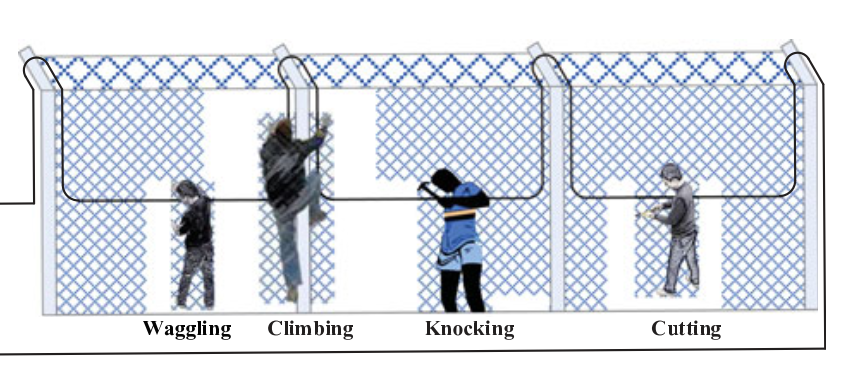
\includegraphics[width=0.7\linewidth]{images/Bab_2/Bab_2_1}
		\caption[Ragam Intrusi]{\small{Sebagian ragam bentuk tindak intrusi}}
	\end{figure}

	\subsection{Serat Optik}
	
	Serat optik merupakan pemandu gelombang silindris dielektrik yang terbuat dari material low-loss seperti plastik maupun gelas silika.
	Serat optik terdiri dari core dimana cahaya dipandu, dan cladding sebagai sebagai selubung core.
	Core memiliki indeks bias lebih tinggi daripada cladding.
	
	\begin{figure}[!ht]
		\centering
		\captionsetup{justification=centering}
		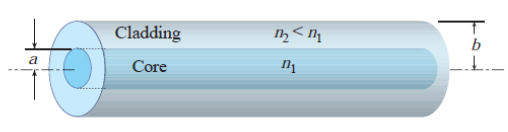
\includegraphics[width=0.7\linewidth]{images/Bab_2/Bab_2_2}
		\caption[Struktur Serat]{\small{Struktur umum serat optik}}
	\end{figure}
	
	Sinar yang masuk pada boundary core-cladding dengan sudut yang lebih besar daripada sudut kritis akan mengalami peristiwa total internal reflection dan akan dipandu melalui core tanpa mengalami pembiasan.
	Berdasarkan moda perambatannaya, serat optik dibagi menjadi dua jenis yaitu serat singlemode yang memiliki diameter core lebih kecil dan serat multimode yang memiliki diameter core lebih besar. 
	Tipe perambatan sinar pada core serat optik dibagi dua yaitu step-index dan graded-index.
	
	\begin{figure}[!ht]
		\centering
		\captionsetup{justification=centering}
		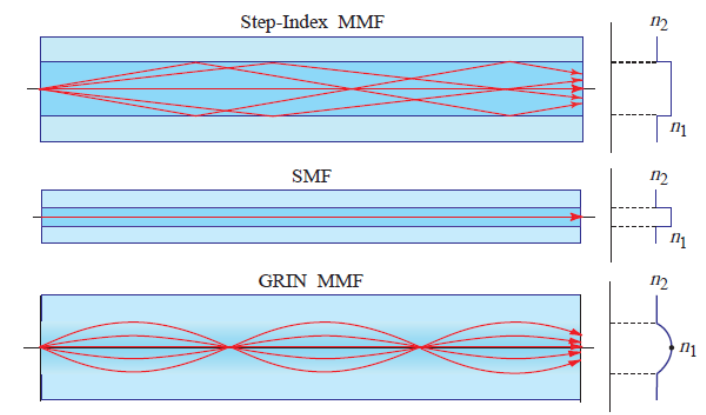
\includegraphics[width=0.7\linewidth]{images/Bab_2/Bab_2_3}
		\caption[Muka Gelombang Serat Optik]{\small{Bentuk Geometri, Profil Indeks Bias dan Tipe Perambatan sinar pada MMF Step, SMF,dan MMF Graded}}
	\end{figure}


	\subsection{Multimode Interference (MMI)}
	
	Multimode Interference (MMI) merupakan fenomena yang terjadi akibat adanya pemantulan cahaya secara berulang didalam susunan core dan cladding pandu gelombang.
	Pemantulan yang berulang didalam core menyebabkan terjadinya interferensi internal, sehingga terjadi perubahan pola cahaya yang keluar dari core secara periodik. 
	Interferensi yang terjadi dapat secara konstruktif maupun destruktif bergantung pada profil indeks bias, jejari, radius, dan panjang gelombang operasi yang digunakan.
	Interferensi konstruktif yang terjadi secara periodik ini disebut sebagai self imaging.
	Fenomena self imaging didalam pandu gelombang multimode dapat dijelaskan menggunakan modal propagation analysis (MPA).
	
	\begin{figure}[!ht]
		\centering
		\captionsetup{justification=centering}
		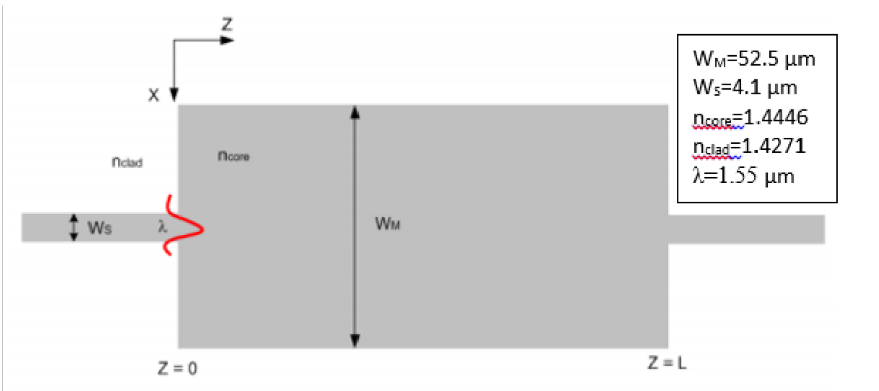
\includegraphics[width=0.7\linewidth]{images/Bab_2/Bab_2_4}
		\caption[Pandu Gelombang SMS]{\small{Skema pandu gelombang multimode pada serat optik SMS}}
	\end{figure}

	Pada profil medan input (z = 0), moda yang berasal dari serat singlemode tereksitasi menjadi distribusi moda yang mungkin terpandu kedalam pandu gelombang serat multimode.
	Sedangkan pada profil medan (z=L), akan menghasilkan self imaging sebanyak n kali dengan jarak tertentu secara periodik (jarak reimaging) .
	Jarak self imaging ditentukan oleh konstanta propagasi antar moda yang berdekatan ($\beta_{m}$ dan $\beta_{m+1}$), dinyatakan sebagai berikut:
	
	\begin{align}
		L_{i} = 10 * \frac{\pi}{\beta_{m} + \beta_{m+1}}
	\end{align}
	
	\subsection{Efek Mekanis pada Serat Optik} 
	
	Efek mekanis disini adalah perlakuan mekanis terhadap serat yang dapat mempengaruhi daya yang dirambatkan oleh serat optik.
	Perlakuan yang dipilih disini adalah macro-bending dimana telah dilakukan penelitian bahwa macro-bending dapat mempengaruhi hasil trace OTDR \cite{Maharinda}.
	
	\subsection{Serat Optik sebagai Distributed Sensor}
	
	Selain sebagai perambat gelombang cahaya, serat optik saat ini juga digunakan sebagai sensor.
	Salah pencapaian dalam serat optik sebagai sensor adalah penggunaannya sebagai distributed sensor \cite{Dakin1992}.
	Pengertian distributed  disini adalah bahwa sepanjang serat optik dapat berfungsi sebagai sensor dan menggantikan model sensor konvensional yang berbasis pengukuran satu titik \cite{Wu2015}.
	Penggunaan distributed sensor ini tentu akan mengurangi biaya dan kompleksitas sistem.
	
	\subsection{Optical Time Domain Reflectometer (OTDR)}
	
	OTDR atau Optical Time Domain Reflectometer adalah alat untuk karakterisasi serat optik yang bekerja dengan mentransmisikan berkas laser dalam bentuk pulsa kemudian mengukur sinyal balik di setiap cacah waktu \cite{test2017}.
	Sinyal balik dalam OTDR merupakan hasil dari fenomena backscattering.
	Skema OTDR secara umum adalah sebagai berikut:
	
	\begin{figure}[!ht]
		\centering
		\captionsetup{justification=centering}
		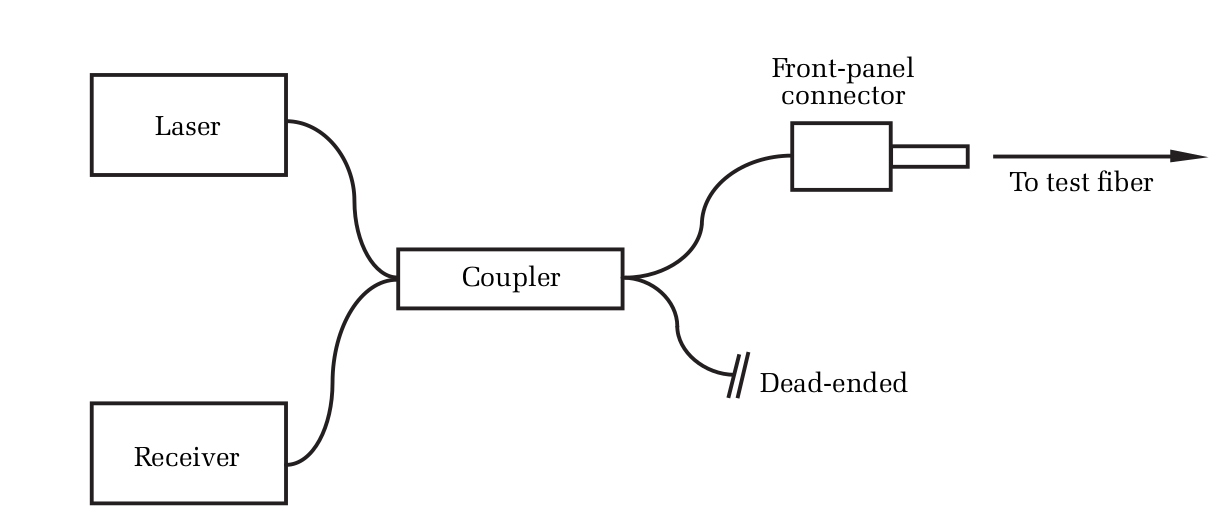
\includegraphics[width=0.65\linewidth]{images/Bab_2/Bab_2_5}
		\caption[Struktur umum OTDR]{\small{Struktur umum OTDR}}
	\end{figure}

	Hasil pengukuran OTDR atau yang sering disebut trace adalah berupa plot nilai pelemahan daya backscatter terhadap waktu atau panjang serat optik \cite{Anderson2004}.
	Berikut adalah tipikal plot trace dalam OTDR:
	
	\begin{figure}[!ht]
		\centering
		\captionsetup{justification=centering}
		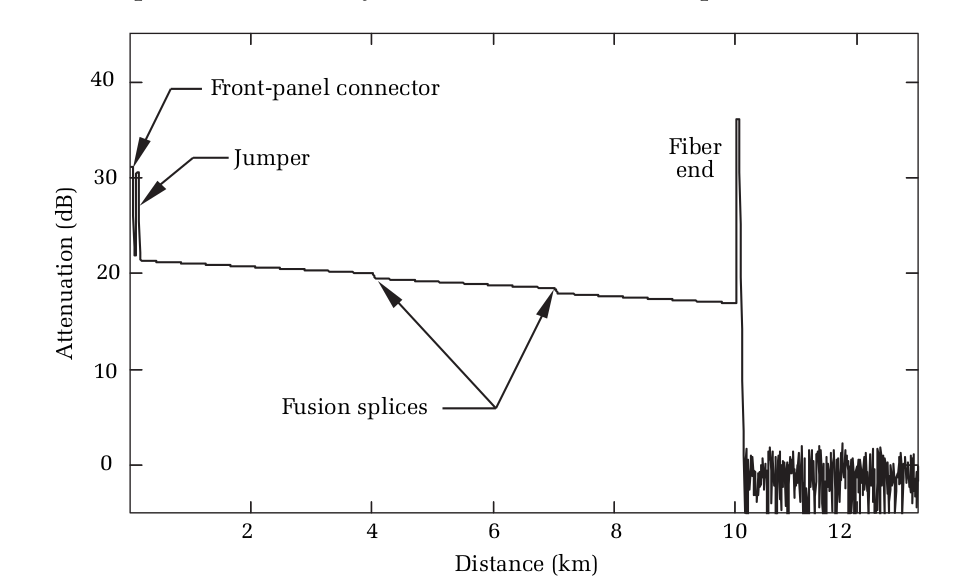
\includegraphics[width=0.7\linewidth]{images/Bab_2/Bab_2_6}
		\caption[Tipikal plot hasil OTDR]{\small{Tipikal plot hasil OTDR}}
	\end{figure}

	Di dalam hasil hasil trace akan menunjukkan respon terhadap events baik berupa reflective maupun non-reflective.
	
	\begin{figure}[!ht]
		\centering
		\captionsetup{justification=centering}
		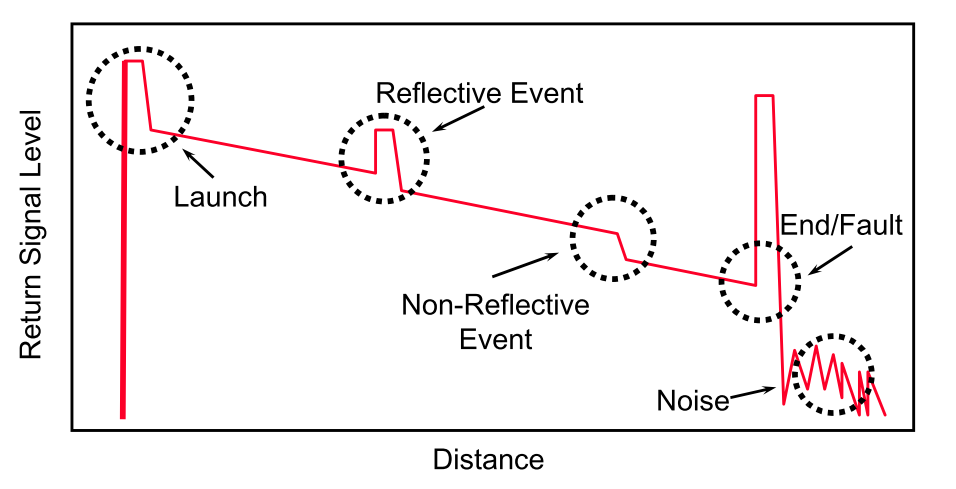
\includegraphics[width=0.7\linewidth]{images/Bab_2/Bab_2_7}
		\caption[respon events hasil OTDR]{\small{respon events hasil OTDR \cite{Anritsu2010}}}
	\end{figure}

	\subsection{Backscattering}
	
	Fenomena backscattering merupakan fenomena yang diakibatkan oleh respon material silikat dari serat optik terhadap pulsa laser yang ditransmisikan oleh OTDR.
	Scattering yang terjadi dapat berupa Raleigh (RB) maupun stimulated Brillouin (SBS) \cite{Feng2017}.
	Berikut adalah skema umum dari backscattering:
	
	\begin{figure}[!ht]
		\centering
		\captionsetup{justification=centering}
		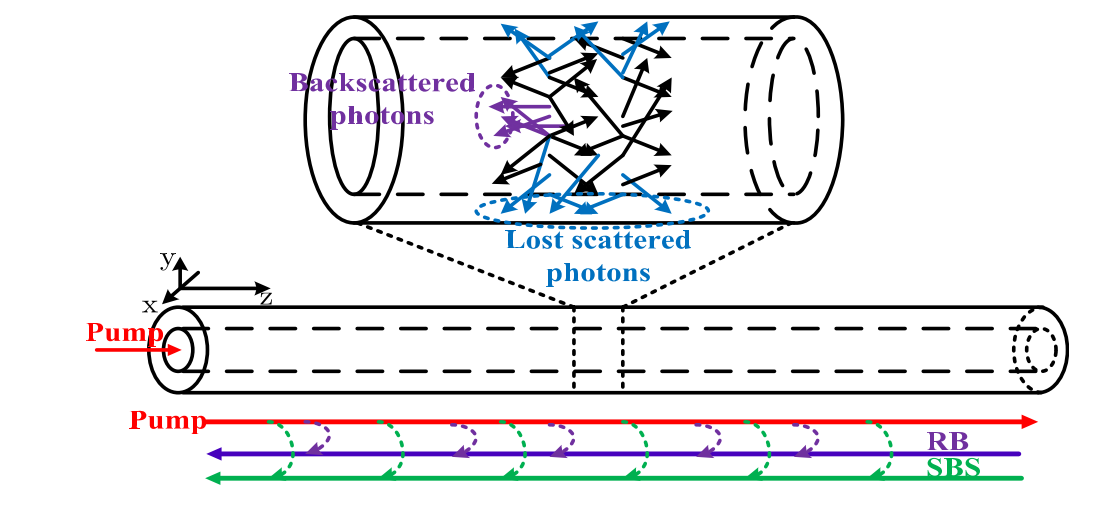
\includegraphics[width=0.4\linewidth]{images/Bab_2/Bab_2_8}
		\caption[Skema umum backscatter.]{\small{Skema umum backscatter.}}
	\end{figure}

	\subsection{Reflective event}

	\subsection{Modul OTDR Anritsu MU909015C}
	
%=============================================================================

%\newpage
%\thispagestyle{plain}
%\mbox{}

%=============================================================================
% BAB III 

\newpage

	\section{Metodologi}
	
	\begin{center}
		{\large \textbf{BAB III}} \\
		{\large \textbf{Metodologi}}
	\end{center}
	
	\subsection{Tempat  Penelitian}
	
	Penelitian ini akan dilakukan di Laboratorium Rekayasa Fotonika Jurusan Teknik Fisika ITS.
	
	\subsection{Prosedur Penelitian}
	
	Prosedur penelitian terdiri dari beberapa tahapan yang dilakukan dari awal hingga akhir untuk tercapainya tujuan dari penelitian ini.
	Metode penelitian merupakan serangkaian kegiatan yang dilakukan dari awal higga akhir untuk tercapainya tujuan penelitian ini.
	
	\begin{figure}[!ht]
		\centering
		\captionsetup{justification=centering}
		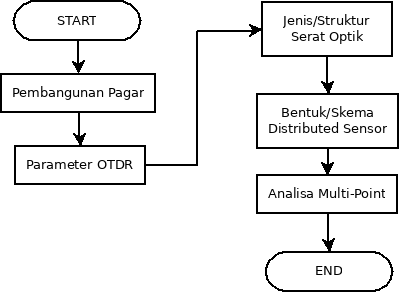
\includegraphics[width=0.4\linewidth]{images/Bab_3/Bab_3_1}
		\caption[Diagram Alir Penelitian]{\small{Diagram Alir Penelitian}}
	\end{figure}

	Prosedur penelitian dibagi menjadi beberapa tahapan yang akan dijelaskan rinci sebagai berikut :
	
	\subsection{Pembuatan Bentang Kawat}
	
	Untuk dapat dilakukan penelitian tentang deteksi intrusi, maka direncanakan perakitan bentang kawat sebagai pengganti pagar.
	Skema akhir seluruhnya mencakup bentang kawat, OTDR, serat optik, gulungan, dan komputer.
	Berikut adalah gambaran setup yang akan dibangun ditunjukkan pada gambar berikut:
	
	\begin{figure}[!ht]
		\centering
		\captionsetup{justification=centering}
		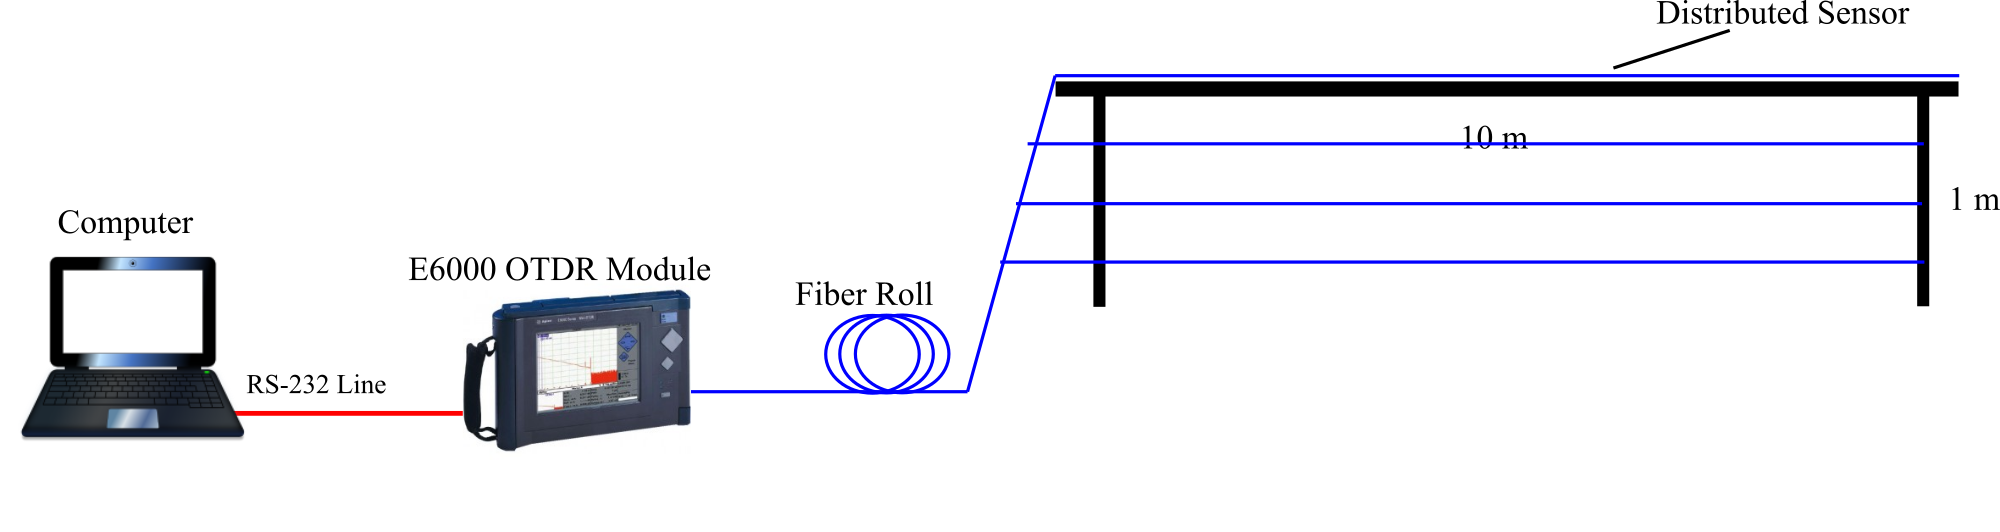
\includegraphics[width=0.8\linewidth]{images/Bab_3/Bab_3_2}
		\caption[Skema Setup]{\small{Skema setup secara global}}
	\end{figure}

	\subsection{Penentuan Parameter OTDR}
	Tahap selanjutnya adalah penentuan nilai parameter OTDR yang dapat menghasilkan hasil trace dengan nilai fluktuasi minimum.
	Parameter yang dimaksud adalah nilai lebar pulsa (\textit{Pulse-Width}) dan periode perataan sample (\textit{averaging}).
	Nilai lebar pulsa yang diuji adalah 5ns, 10ns, 20ns, 50ns, dan 100ns.
	Sedangkan untuk perataan sample adalah untuk setiap 1s, 5s, 10s, 15s, 30s, 45s, dan 60s.
	Penentuan nilai-nilai parameter ini dapat dilakukan di module sendiri melalui software antar muka pada module OTDR.
	
	\begin{figure}[!ht]
		\centering
		\captionsetup{justification=centering}
		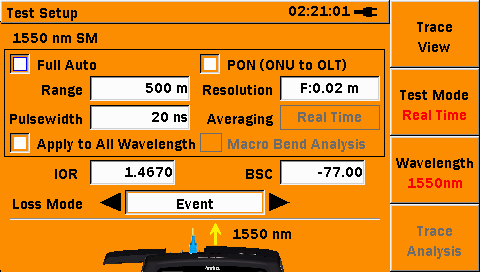
\includegraphics[width=0.5\linewidth]{images/Bab_3/Bab_3_4}
		\caption[panel antar-muka module]{\small{Panel antar-muka module }}
	\end{figure}

	Dalam eksperimen ini digunakan parameter OTDR nilai Index of Reflection (IOR) sebesar 1.4670 dan BackScatter Coefficient (BSC) senilai -77 \cite{Hafid2014}.
	Sedangkan untuk panjang gelombang digunakan 1550 nm karena panjang gelombang ini peka terhadap gangguan. 

	\subsection{Uji Gangguan Displacement}
	
	Dengan memperhatikan setiap hasil uji perlakukan sebelumnya, maka selanjutnya dilakukan uji eksperimen displacement dengan bantuan kawat sebagai pengganti pagar. 
	Konfigurasi yang dipilih adalah Singlemode-Multimode-Singlemode.
	Setup yang dilakukan adalah dengan membentangkan kawat yang disatukan dengan serat optik, kemudian dilakukan uji \textit{bending} atau \textit{displacement}.\cite{Tian2017}\cite{Gong2011}\cite{Arifin2015} 
	Panjang yang digunakan adalah 1 meter dan 5 meter mengingat standar panjang unit pagar adalah 2,4 meter.\cite{Pagar2015}
	
	Berikut adalah setup pengujian:
	
	\begin{figure}[!ht]
		\centering
		\captionsetup{justification=centering}
		\begin{subfigure}[b]{0.3\textwidth}
			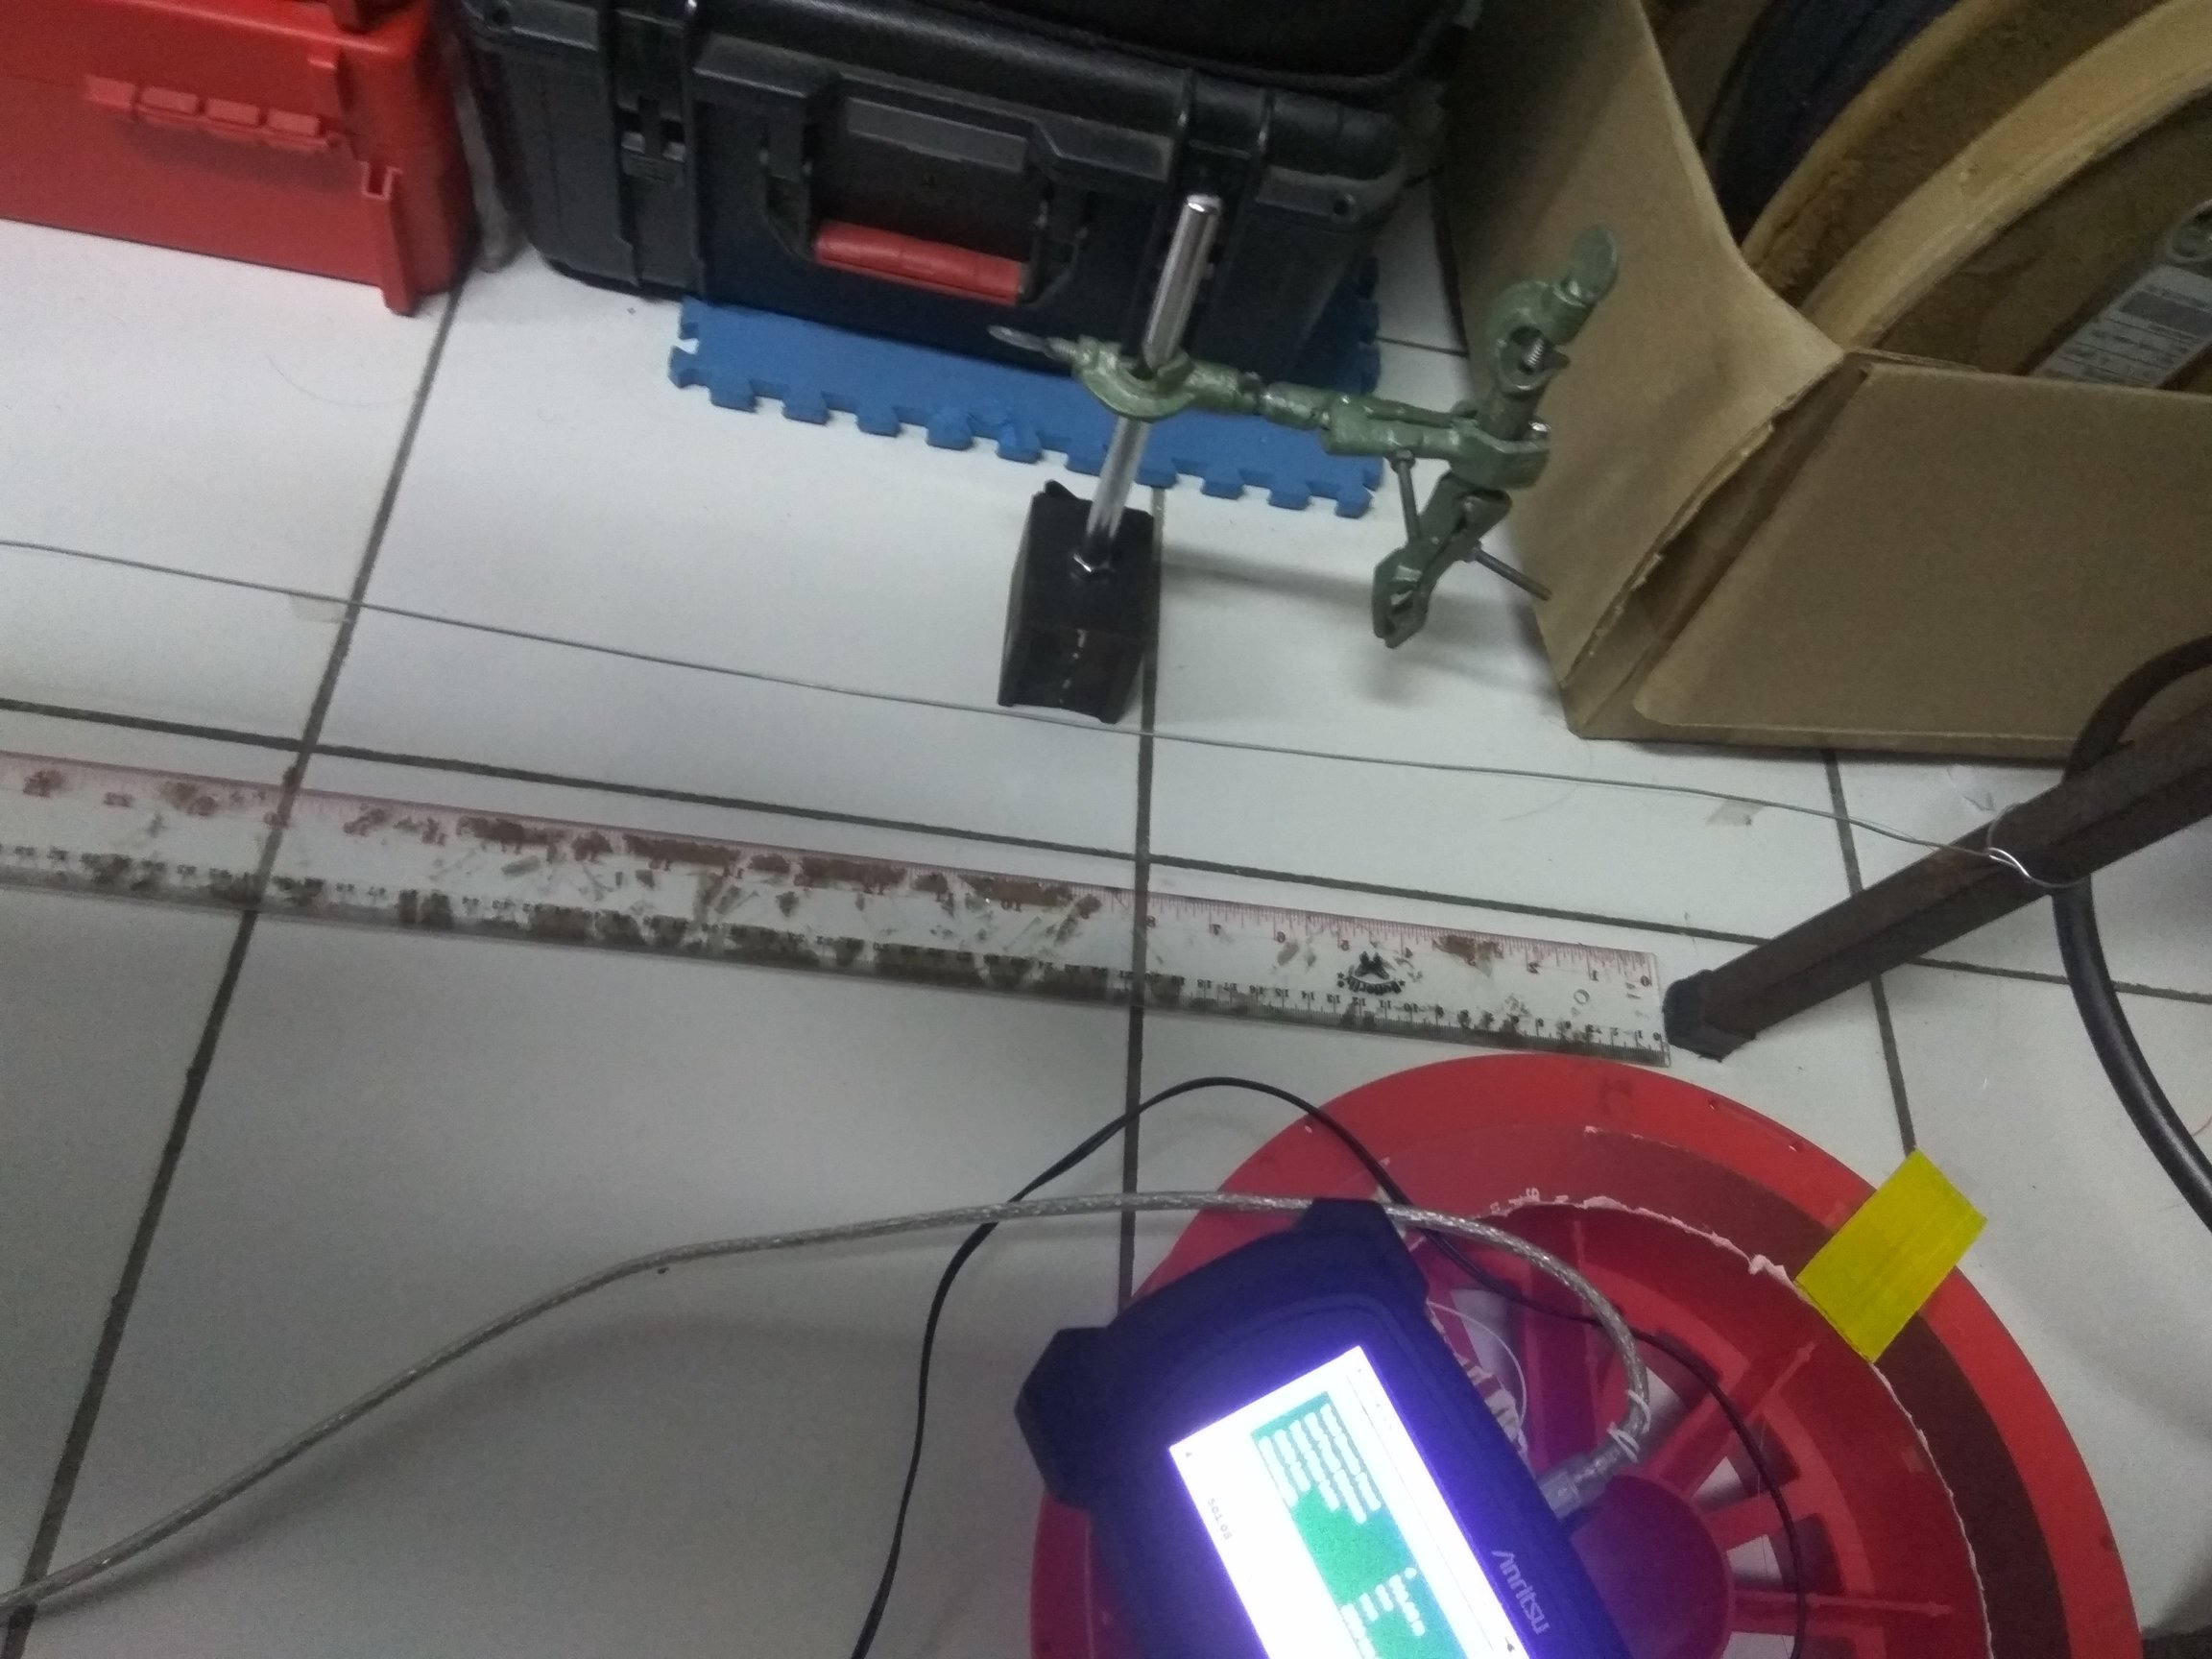
\includegraphics[width=\textwidth]{images/Bab_4/Bab_4_5a}	
			\caption{\small{Ujung awal dan OTDR}}		
		\end{subfigure}
		\begin{subfigure}[b]{0.3\textwidth}
			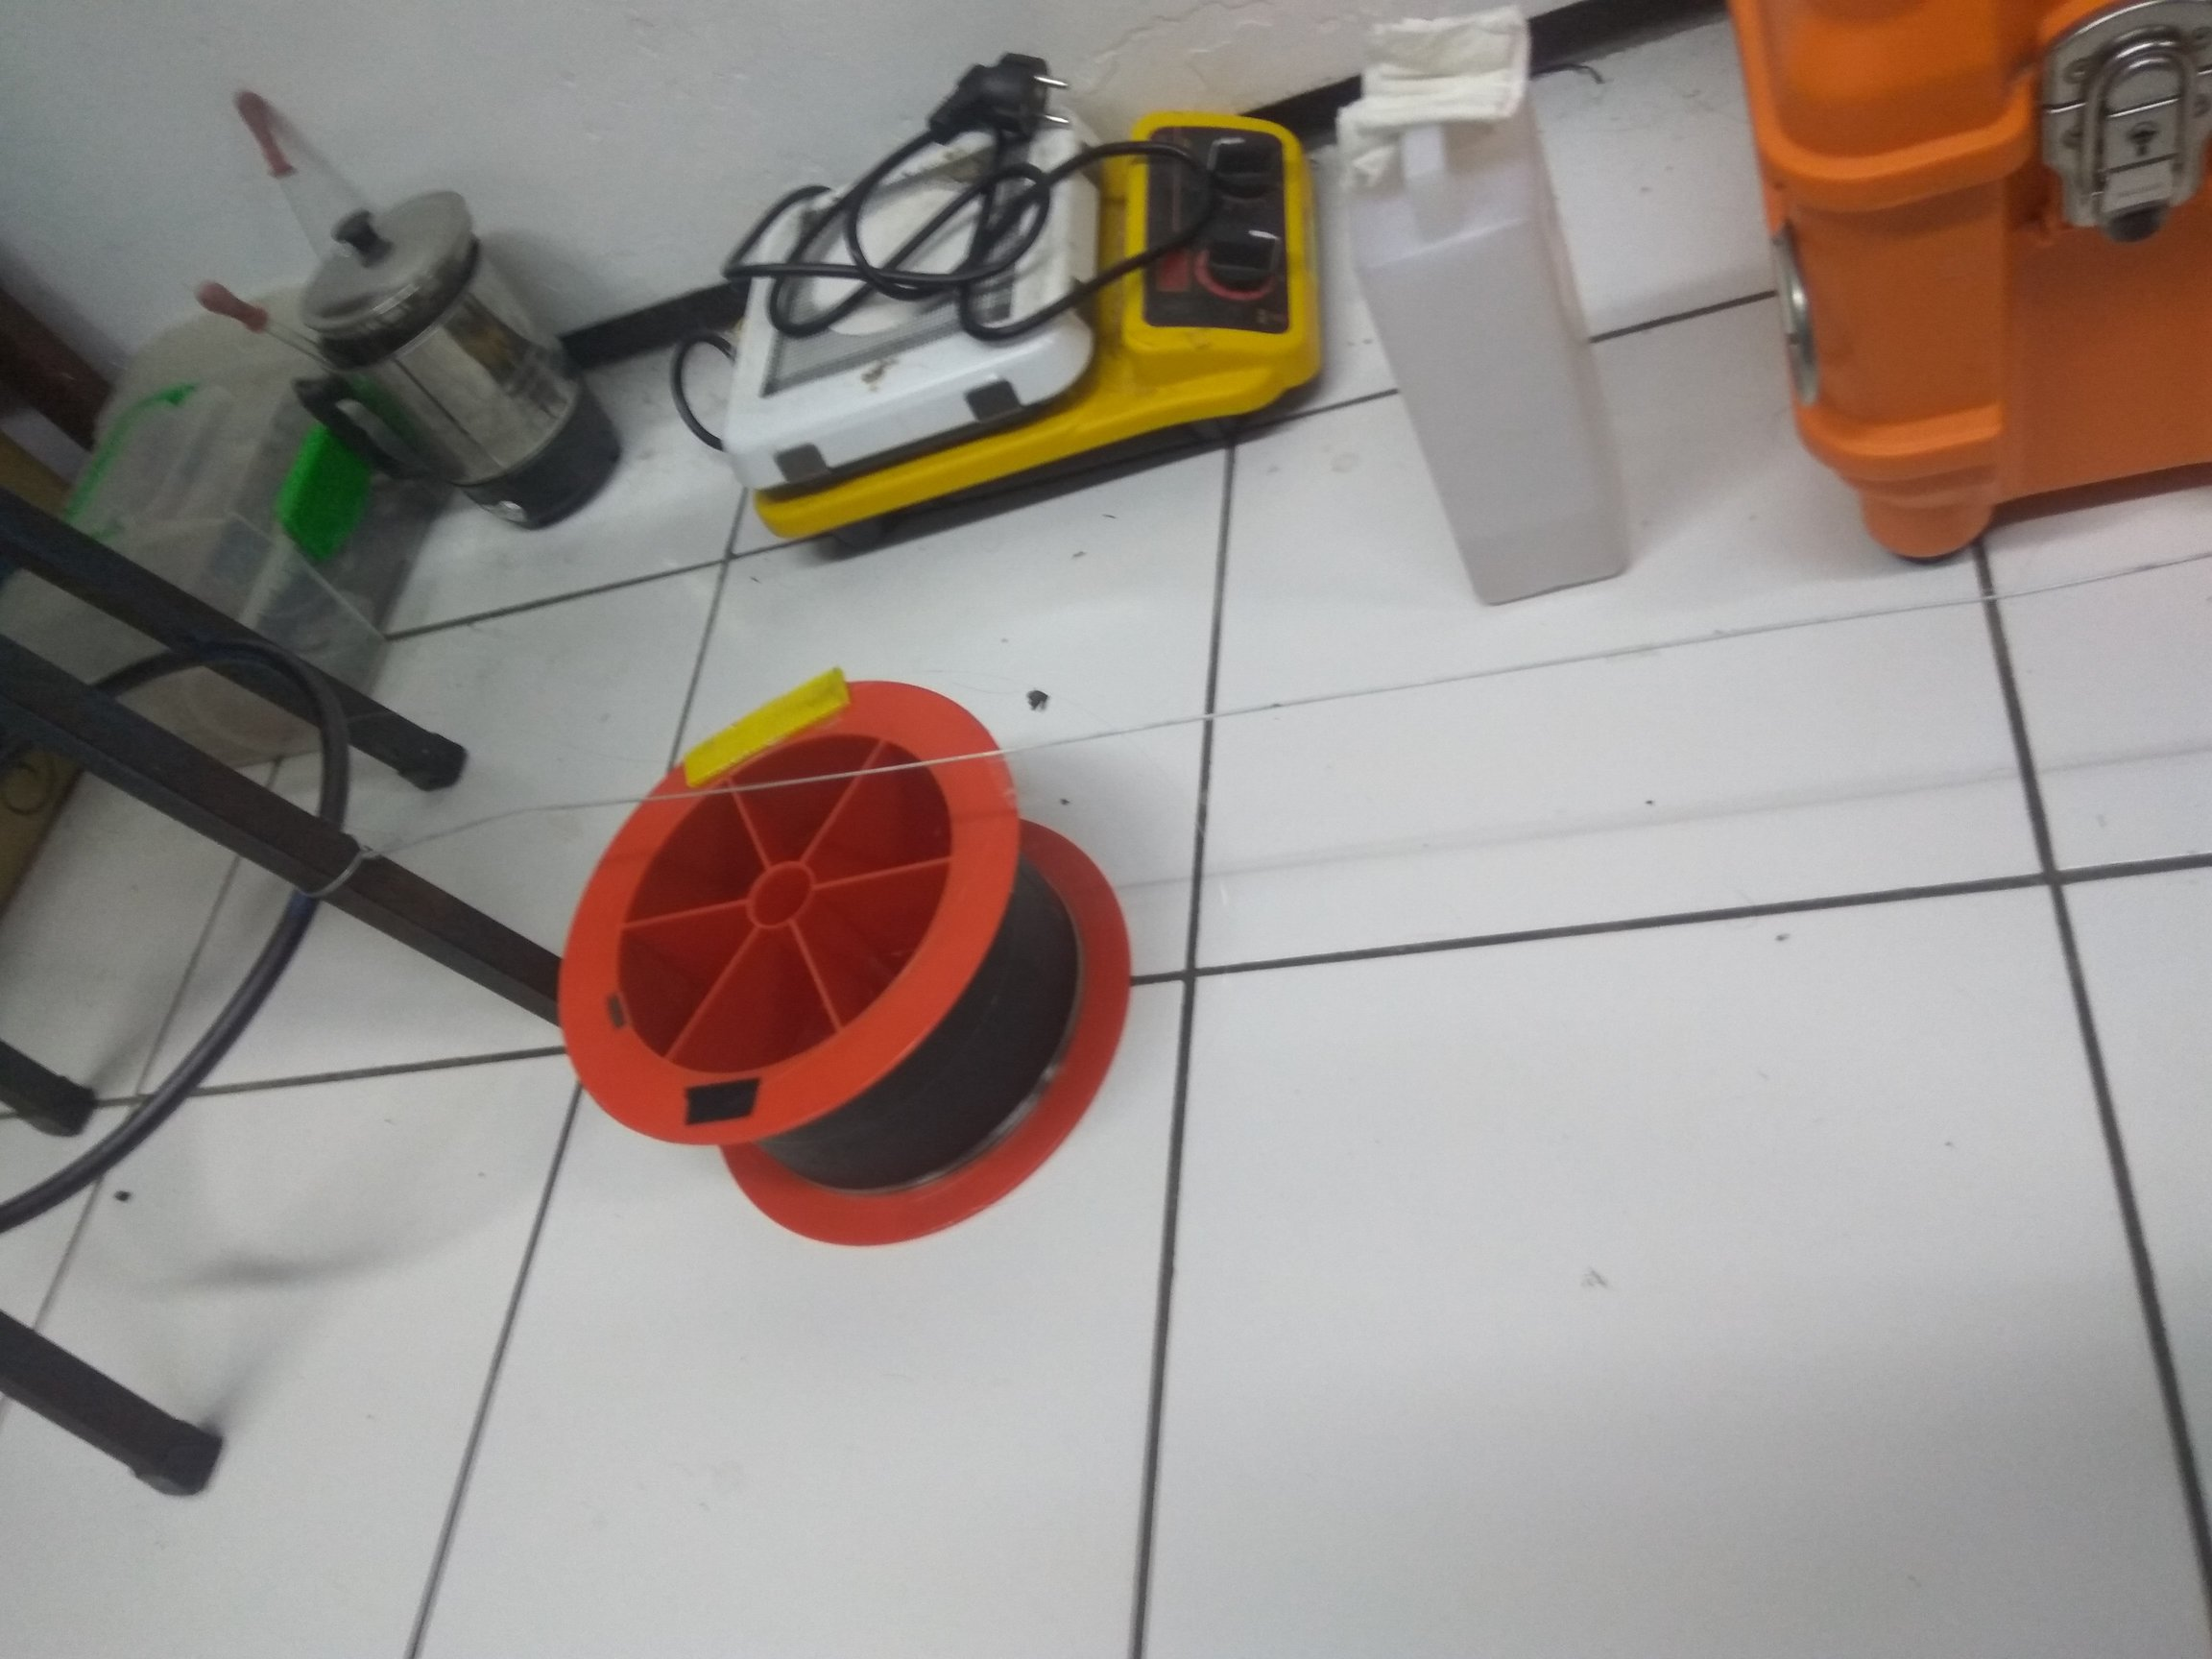
\includegraphics[width=\linewidth]{images/Bab_4/Bab_4_5b}
			\caption{\small{Ujung akhir}}			
		\end{subfigure}
		\begin{subfigure}[b]{0.4\textwidth}
			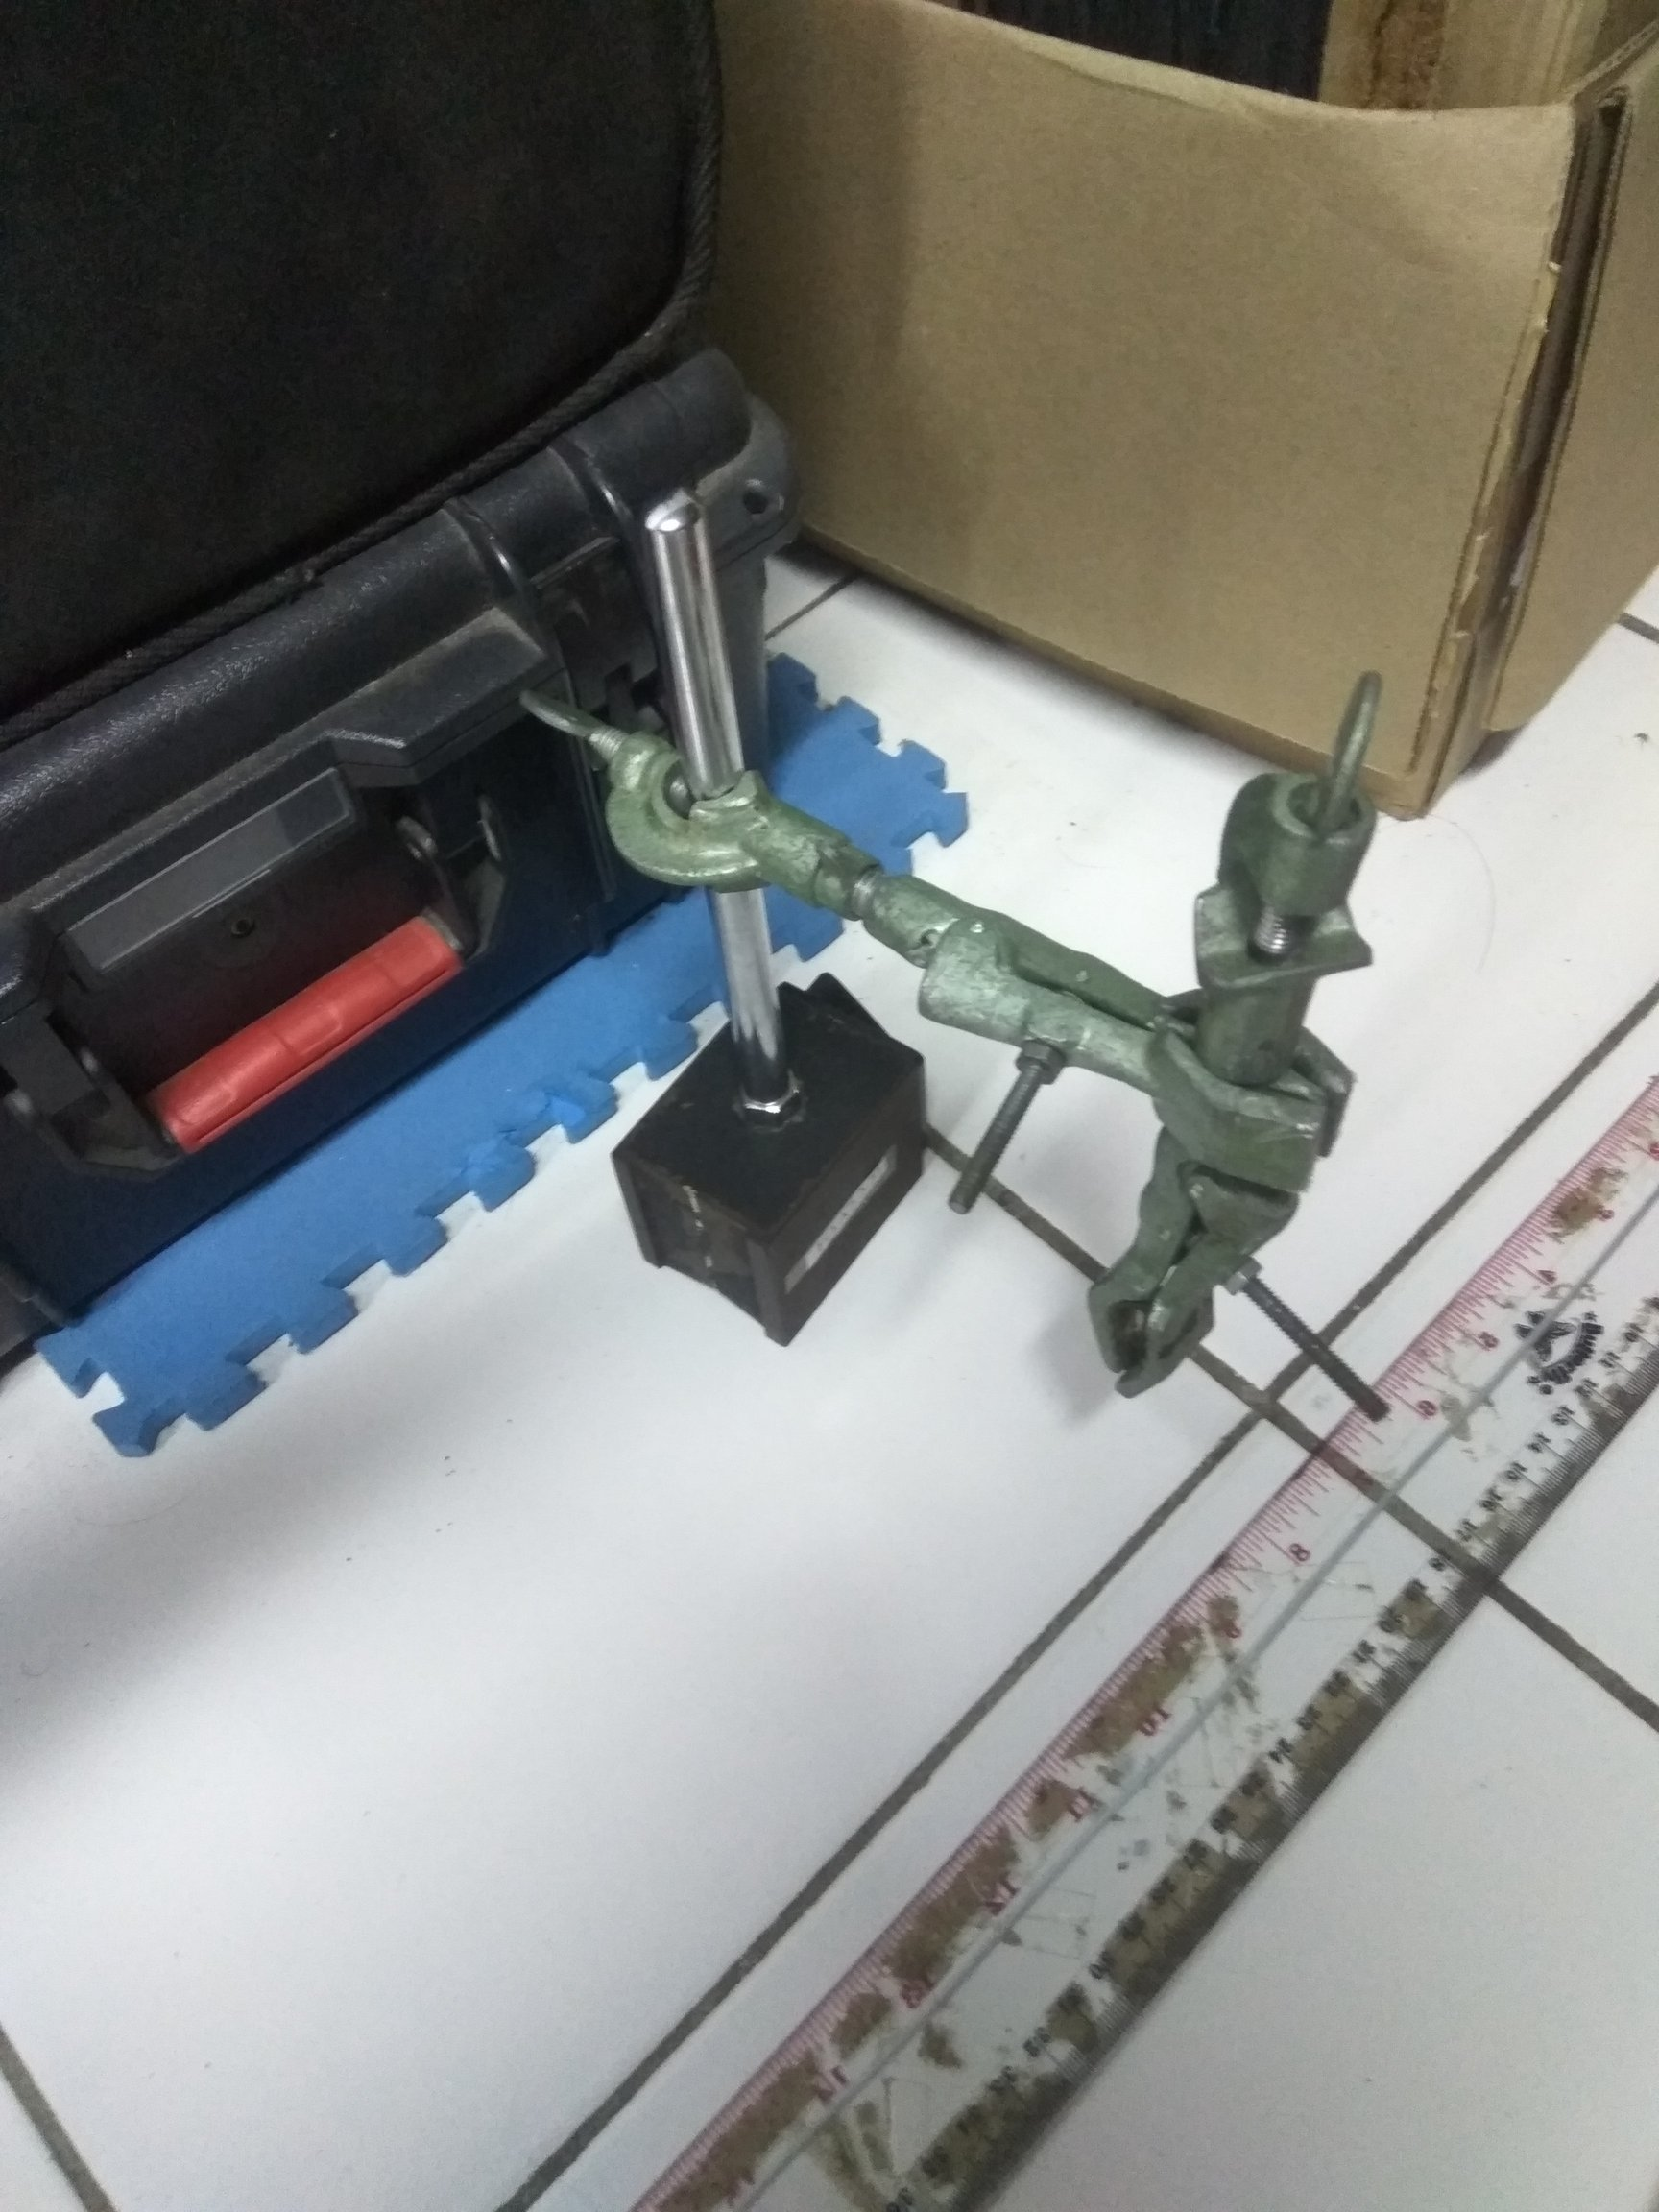
\includegraphics[width=\linewidth]{images/Bab_4/Bab_4_5c}
			\caption{\small{Statif dan holder untuk \textit{bending/displacement}}}			
		\end{subfigure}
		\caption[Uji Pagar]{\small{Gambaran Uji Gangguan Pagar }}
	\end{figure}
	
	Sedangkan \textit{displacement} yang dilakukan adalah sejauh 5mm, 10mm, 15mm, 20mm, dan 25mm vertikal ke bawah.
	Nilai yang diperhatikan adalah nilai puncak pada dua event, yaitu
	
	\begin{itemize}
		\item fiber \textit{splice}, yaitu \textit{splice} antara singlemode dan multimode  
		\item fiber \textit{splice}, yaitu \textit{splice} antara multimode dan singlemode.
		Splice kedua ini hanya muncul pada setup fiber 5 meter 
		\item fiber \textit{end}, yaitu ujung akhir fiber singlemode terakhir.
	\end{itemize}
	
	Sedangkan posisi displacement adalah setiap penambahan jarak konstan 20cm.

	\subsection{Analisa Multi-Point}
	
	Tahapan terakhir dalam penelitian ini adalah tahap analisa hasil trace untuk menentukan	resspon pada pagar secara akurat.
	Analisa dilakukan dengan mengambil hasil trace sebagai sinyal periodik domain waktu untuk mendapatkan jumlah titik dengan amplitudo yang tergolong events.
	Hasil analisa ini kemudian digeneralisasi sehingga dapat dituangkan ke dalam bentuk algoritma yang dapat digunakan untuk menghitung jumlah gangguan.
	
	Sebelum melakukan analisa, maka perlu dilakukan konversi format data dari standar data Bellcore (*.sor) menjadi data array yang dapat dibaca oleh interpreter Matlab/Python (*.dat).
	Metode konversi yang dipilih menggunakan modul Python pyOTDR (\url{https://github.com/sid5432/pyOTDR}) bersama modul olahdata seperti NumPy dan SciPy.
	Kemudian untuk proses konversi menggunakan skrip sebagai berikut:
	
	\begin{minted}[frame=lines,fontsize=\footnotesize]{bash}
#!/bin/bash

for i in `ls *.sor`;do
echo "converting $i"
pyOTDR $i > /dev/null
done

echo "removing all JSON data"
rm -f *.json
	\end{minted}
	
	Selanjutnya langkah terakhir adalah pencarian nilai rata sekaligus plot grafik.
	Bahasa yang digunakan adalah Python bersama dengan modul Numpy dan Matplotlib.
	
	\begin{minted}[frame=lines,fontsize=\footnotesize]{python}
#!/usr/bin/python

import numpy as np
import matplotlib.pyplot as plt
	\end{minted}
	
	Data array terbagi dalam 2 kategori, yaitu data posisi gangguan (dalam centimeter) senilai 0,20,40,60, dan 80, dan data nilai kedalaman gangguan (dalam mm) senilai 5, 10, 15, 20, dan 25.

	\begin{minted}[frame=lines,fontsize=\footnotesize]{python}
pos = ['20','40','60','80']
vpos = [0,20,40,60,80]
place = ['05','10','15','20','25']

vdispos = [0,20,40,60,80]
vdisval = [5,10,15,20,25]
	\end{minted}
	
	Untuk data \textit{chunk} (potongan data), terdapat dua varian, yaitu data untuk posisi splice (array 3500 hingga 4500) dan untuk posisi end (array 4500 hingga 5500).
	Untuk nilai dasar (tanpa gangguan) didapat melalu skrip berikut:
	
	\begin{minted}[frame=lines,fontsize=\footnotesize]{python}
A_start = 3500
A_end = 4500

data_base = (
	np.genfromtxt('data_1_base_a-trace.dat')[A_start:A_end,1] +
	np.genfromtxt('data_1_base_b-trace.dat')[A_start:A_end,1] +
	np.genfromtxt('data_1_base_c-trace.dat')[A_start:A_end,1])/3

max_base = np.max(data_base)
	\end{minted}
	
	Variabel data\_base adalah semua nilai array sedangkan untuk max\_base adalah nilai	maximal array tersebut.
	Dengan pola yang sama, maka untuk mendapatkan array dan nilai maximum menggunakan skrip:
	
	\begin{minted}[frame=lines,fontsize=\footnotesize]{python}
for i in pos:
	for j in place:
		filepath_a = 'data_1_%s_%s_a-trace.dat' % (i,j)
		filepath_b = 'data_1_%s_%s_b-trace.dat' % (i,j)
		filepath_c = 'data_1_%s_%s_c-trace.dat' % (i,j)
		
		globals()['data_%s_%s' % (i,j)] = (
			np.genfromtxt(filepath_a)[A_start:A_end,1] +
			np.genfromtxt(filepath_b)[A_start:A_end,1] +
			np.genfromtxt(filepath_c)[A_start:A_end,1])/3
		
		globals()['d_%s_%s' % (i,j)] = np.abs(
			np.max(globals()['data_%s_%s' % (i,j)]) - max_base)
	\end{minted}
	
	Selanjutnya semua nilai maximum digabungan dengan array nilai kedalaman gangguan:
	
	\begin{minted}[frame=lines,fontsize=\footnotesize]{python}
displace_05 = np.zeros(1)
displace_10 = np.zeros(1)
displace_15 = np.zeros(1)
displace_20 = np.zeros(1)
displace_25 = np.zeros(1)
	
for i in place:            
	for j in pos:
		globals()['displace_%s' % i] = np.append(
			[globals()['displace_%s' % i]],
			[globals()['d_%s_%s' % (j,i)]])
	\end{minted}
	
	dan terakhir adalah plot grafik:
	
	\begin{minted}[frame=lines,fontsize=\footnotesize]{python}
plt.figure()
plt.xlabel('position (cm)')
plt.ylabel('delta-power (dB)')
plt.plot(vpos,displace_05,'ro-',label='5mm')
plt.legend(loc='best')
	\end{minted}

%=============================================================================

\newpage
\thispagestyle{plain}
\mbox{}
	
%=============================================================================
%% BAB IV
\newpage
	
	\section{Hasil dan Pembahasan}
	
	\begin{center}
		{\large \textbf{BAB IV}} \\
		{\large \textbf{Hasil dan Pembahasan}}
	\end{center}
	
	\subsection{Hasil uji di parameter OTDR}
	
	Berikut disajikan grafik sebagai komparasi nilai standar deviasi untuk setiap 10 sampel pada kategori selang averaging dan lebar pulsa berbeda-beda.
	Dengan hasil ini maka pengujian selanjutnya akan mengacu pada nilai averaging dan lebar pulsa paling rendah.
	
	\begin{figure}[!ht]
		\centering
		\captionsetup{justification=centering}
		\begin{subfigure}[b]{0.7\textwidth}
			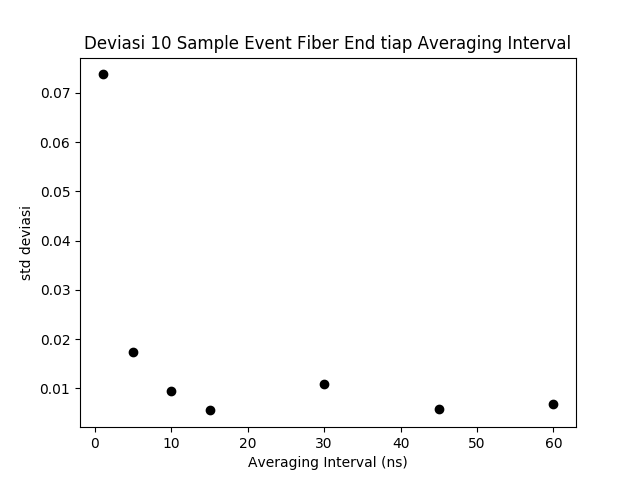
\includegraphics[width=\textwidth]{images/Bab_4/stddev_avg_end}	
			\caption{\small{standar deviasi setiap variasi averaging pada fiber end}}		
		\end{subfigure}
		\begin{subfigure}[b]{0.7\textwidth}
			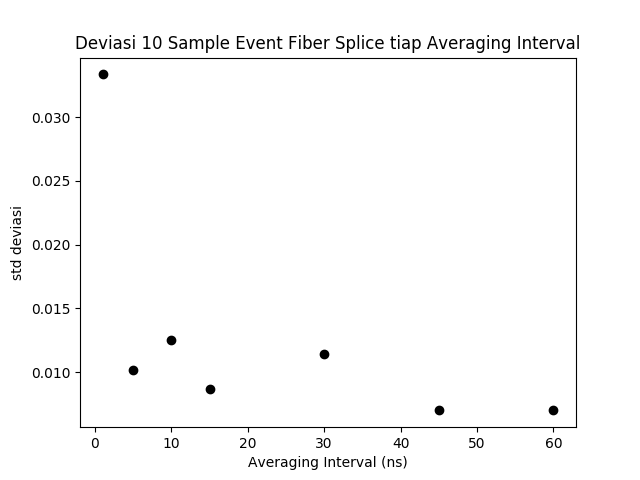
\includegraphics[width=\linewidth]{images/Bab_4/stddev_avg_splice}
			\caption{\small{standar deviasi setiap variasi averaging pada fiber splice}}			
		\end{subfigure}
		\caption[belum ada judul]{\small{standar deviasi setiap variasi averaging}}
	\end{figure}

	Dengan memperhatikan dua grafik tersebut, dapat diketahui bahwa semakin lama selang averaging, maka semakin kecil deviasi untuk pengukuran berulang.
	Hal ini dapat dipahami karena semakin lama selang averaging, maka semakin banyak sampel yang dirata-ratakan, sehingga fluktuasi pengukuran semakin kecil.

	\begin{figure}[!ht]
		\centering
		\captionsetup{justification=centering}
		\begin{subfigure}[b]{0.7\textwidth}
			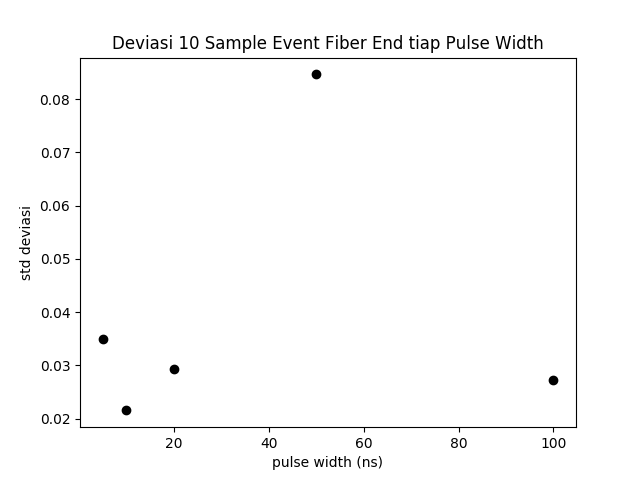
\includegraphics[width=\textwidth]{images/Bab_4/stddev_pw_end}	
			\caption{\small{standar deviasi setiap variasi lebar pulsa pada fiber end}}		
		\end{subfigure}
		\begin{subfigure}[h]{0.7\textwidth}
			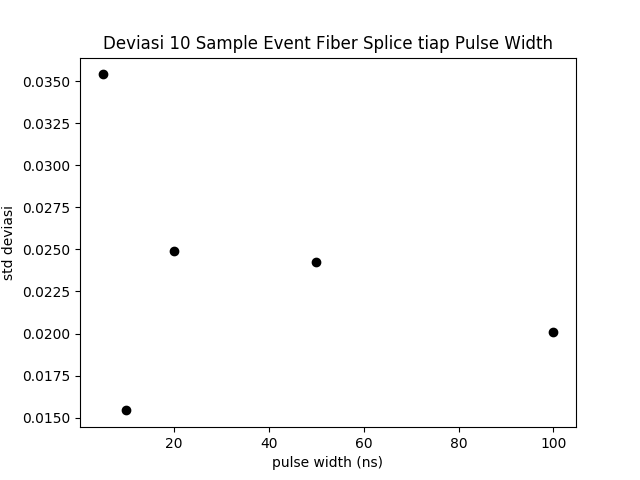
\includegraphics[width=\linewidth]{images/Bab_4/stddev_pw_splice}
			\caption{\small{standar deviasi setiap variasi lebar pulsa pada fiber splice}}			
		\end{subfigure}
		\caption[belum ada judul]{\small{standar deviasi setiap variasi lebar pulsa}}
	\end{figure}

	Selanjutnya dengan memperhatikan dua grafik di atas, dapat diketahui bahwa tidak setiap penambahan lebar pulsa akan berpengaruh terhadap fluktuasi respon.
	
	\newpage
	\subsection{Hasil uji di setiap konfigurasi serat optik}
	
	Berikut dipaparkan hasil setiap konfigurasi disertai pembandingan, sehingga dapat diketahui perbedaan respon OTDR di setiap perlakuan.
	
	\begin{enumerate}
		\item \textbf{Single Mode}

		Konfigurasi pertama yang diambil trace adalah serat optik SingleMode.
		Pada konfigurasi ini, tidak diberikan gangguan untuk menjadi acuan dasar.
		Berikut skema konfigurasi:
		
		\begin{figure}[!ht]
			\centering
			\captionsetup{justification=centering}
			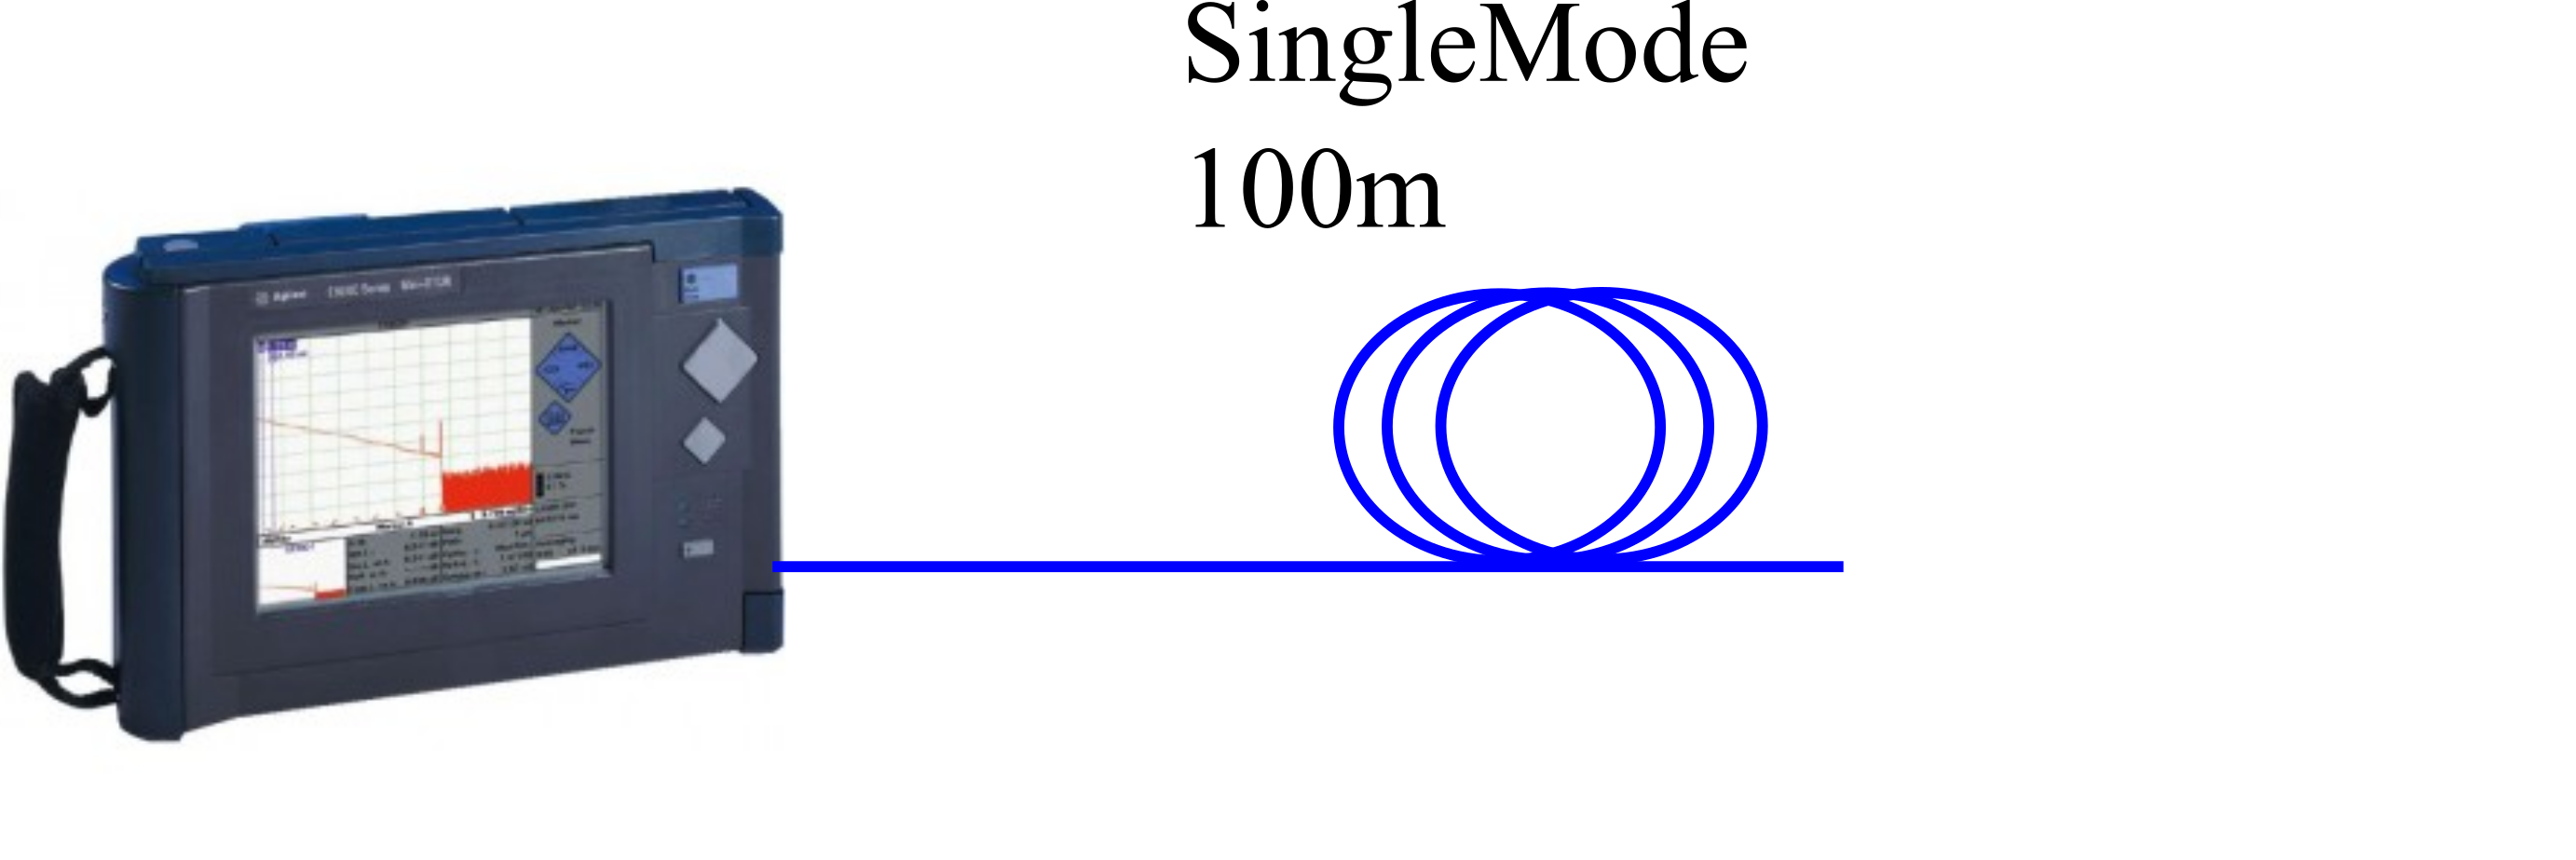
\includegraphics[width=0.6\linewidth]{images/Bab_4/s_basic}
			\caption[Trace SMF-SMF]{\small{Rangkaian serat optik SingleMode}}
		\end{figure}
	
		dan berikut adalah hasil trace OTDR untuk serat optik SMF dengan satu splice yaitu antara 1 roll SMF 100m dengan 10 cm SMF dengan konektor FC (pigtailed)
		
		\begin{figure}[!ht]
			\centering
			\captionsetup{justification=centering}
			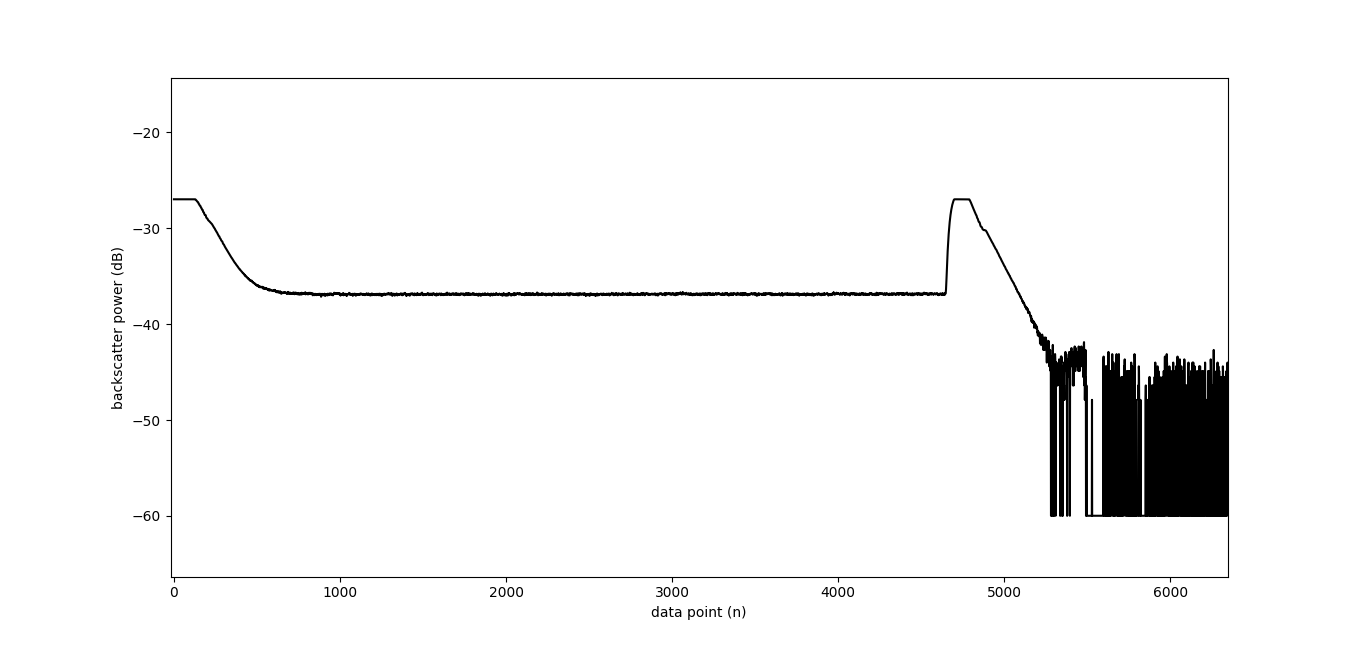
\includegraphics[width=\linewidth]{images/Bab_4/Bab_4_3a1}
			\caption[Trace SMF]{\small{Hasil trace OTDR pada SMF normal}}
		\end{figure}
	
		Apabila diperhatikan, maka grafik diatas terdiri dari 4 bagian, yaitu:
		\begin{itemize}
			\item Event Coupling, yaitu event akibat adanya kopling melalui konektor FC.
			\item Trace sepanjang fiber optik.
			\item Event Reflective, yaitu event akibat adanya perbedaan indeks bias yang signifikan di ujung fiber.
			\item Trace Noise, yaitu noise akibat panjang serat optik telah berakhir.
		\end{itemize}
		
		\newpage
		\item \textbf{Single Mode – Single Mode}
		
		Berikut adalah hasil trace OTDR untuk serat optik SMF dengan dua splice yaitu antara 1 roll SMF 100m, 1 roll SMF 50m, dan 10 cm SMF dengan konektor FC (pigtailed).
		
		Skema rangkaian serat optik (segmen merah adalah yang mendapat gangguan):
		
		\begin{figure}[!ht]
			\centering
			\captionsetup{justification=centering}
			\includegraphics[width=0.6\linewidth]{images/Bab_4/sm}
			\caption[Trace SMF-SMF]{\small{Rangkaian serat optik SingleMode-SingleMode}}
		\end{figure}
	
		Selanjutnya berikutnya adalah grafik hasil trace OTDR kondisi tanpa gangguan:
		
		\begin{figure}[!ht]
			\centering
			\captionsetup{justification=centering}
			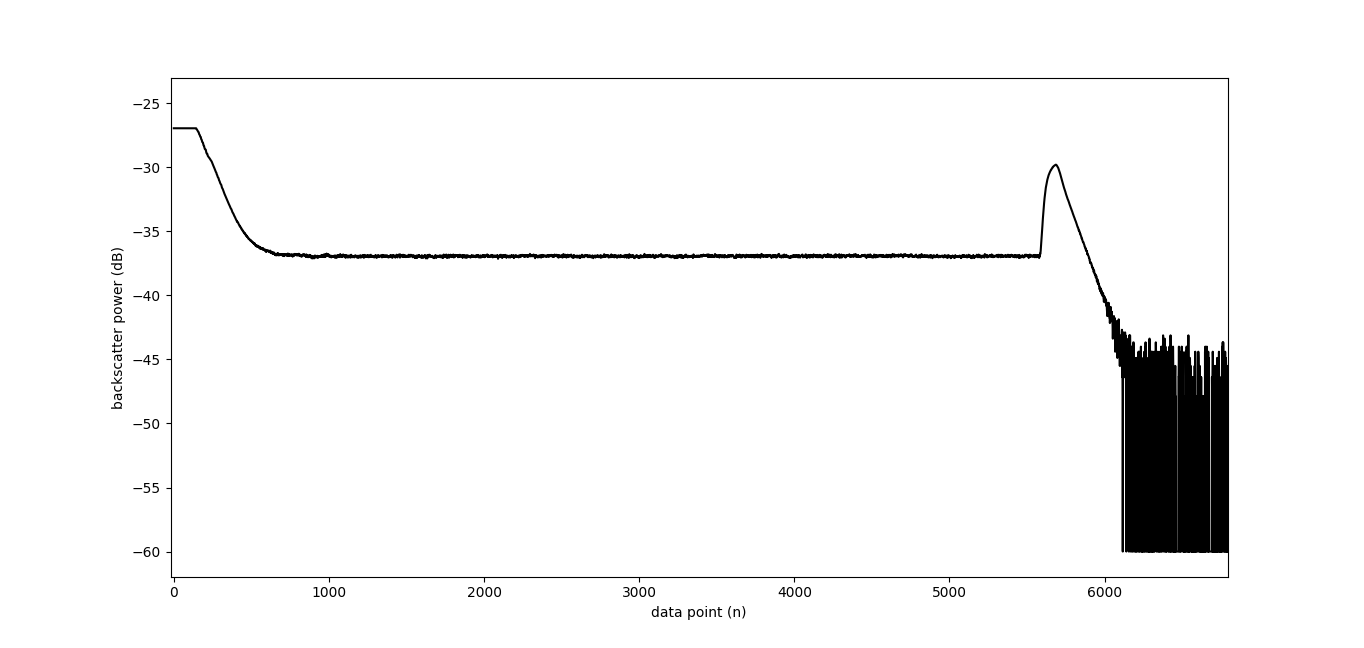
\includegraphics[width=\linewidth]{images/Bab_4/Bab_4_3b1}
			\caption[Trace SMF-SMF]{\small{Hasil trace OTDR pada SM-SM normal}}
		\end{figure}
	
		dan berikutnya adalah grafik hasil trace OTDR kondisi dengan gangguan:
		
		\begin{figure}[!ht]
			\centering
			\captionsetup{justification=centering}
			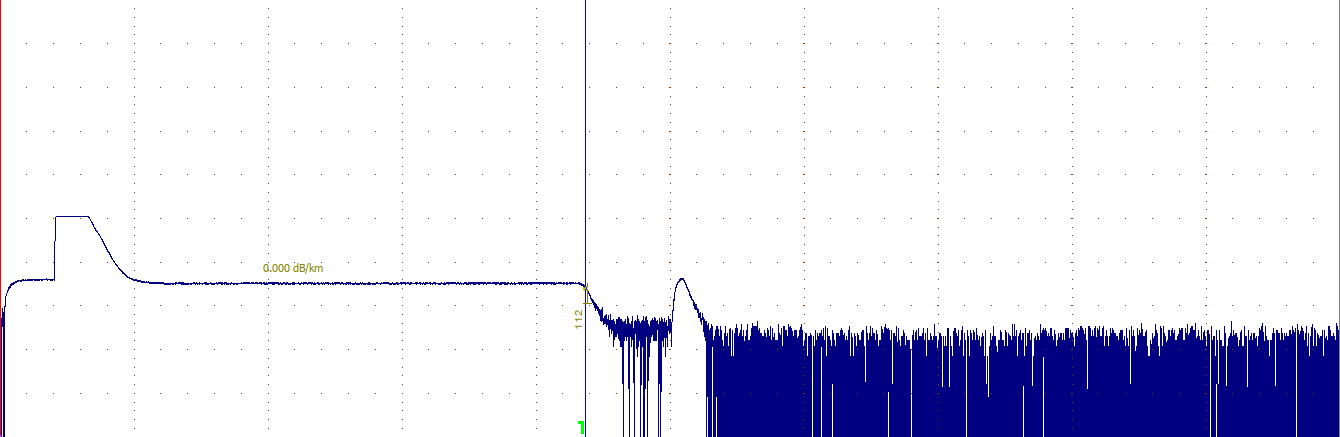
\includegraphics[width=\linewidth]{images/Bab_4/Bab_4_3b2}
			\caption[Trace SMF-SMF]{\small{Hasil trace OTDR pada SM-SM dengan gangguan}}
		\end{figure}
	
		Apabila kedua grafik dibandingkan, maka perubahannya yang dapat terlihat adalah turunnya daya pada event ujung fiber.
		Sedangkan pada bagian lainnya didapatkan identik. 
		Berikut adalah grafiknya (grafik hitam adalah kondisi tanpa gangguan):
		
		\begin{figure}[!ht]
			\centering
			\captionsetup{justification=centering}
			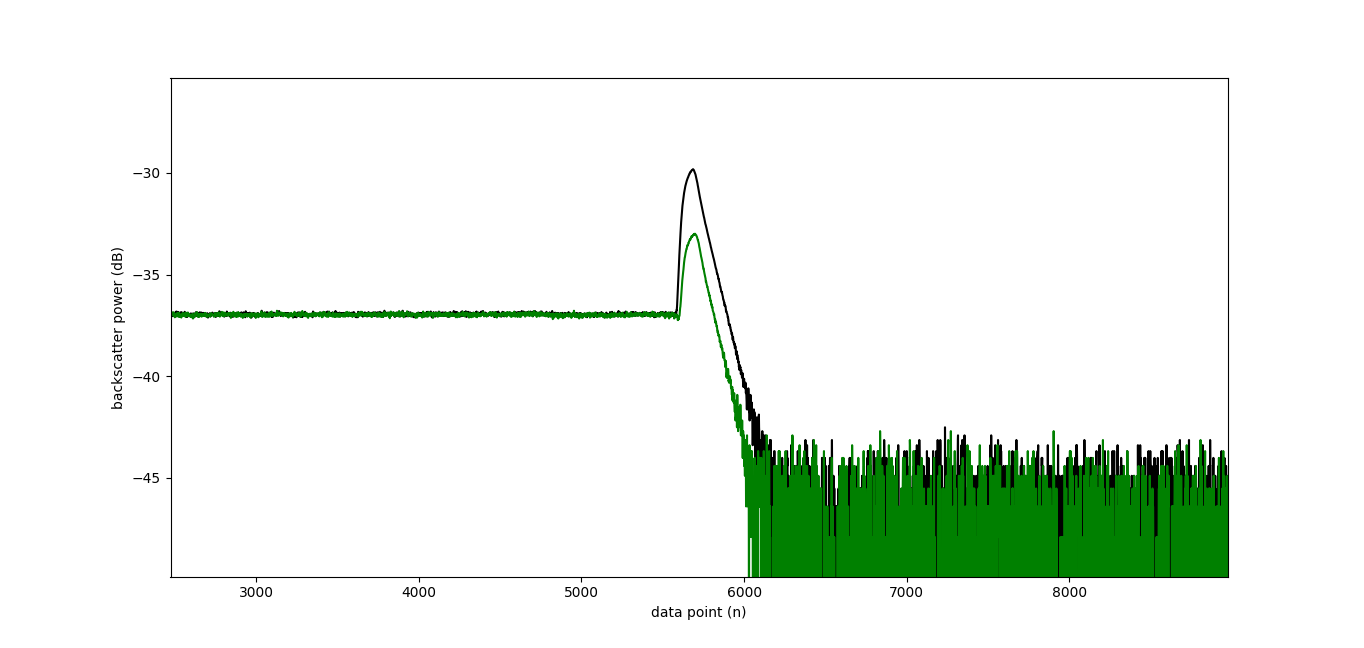
\includegraphics[width=0.8\linewidth]{images/Bab_4/Bab_4_3b3}
			\caption[Trace SMF-SMF]{\small{Komparasi kedua grafik pada bagian event ujung fiber}}
		\end{figure}
		
		\item \textbf{Single Mode – Multi Mode Graded Index}
		
		Berikut adalah hasil trace OTDR untuk serat optik SMF dengan dua splice yaitu antara 1 roll SMF 100m, 1 roll MMF-GI 100m, dan 10 cm SMF dengan konektor FC (pigtailed).
		Skema rangkaian serat optik (segmen merah adalah yang mendapat gangguan):
		
		\begin{figure}[!ht]
			\centering
			\captionsetup{justification=centering}
			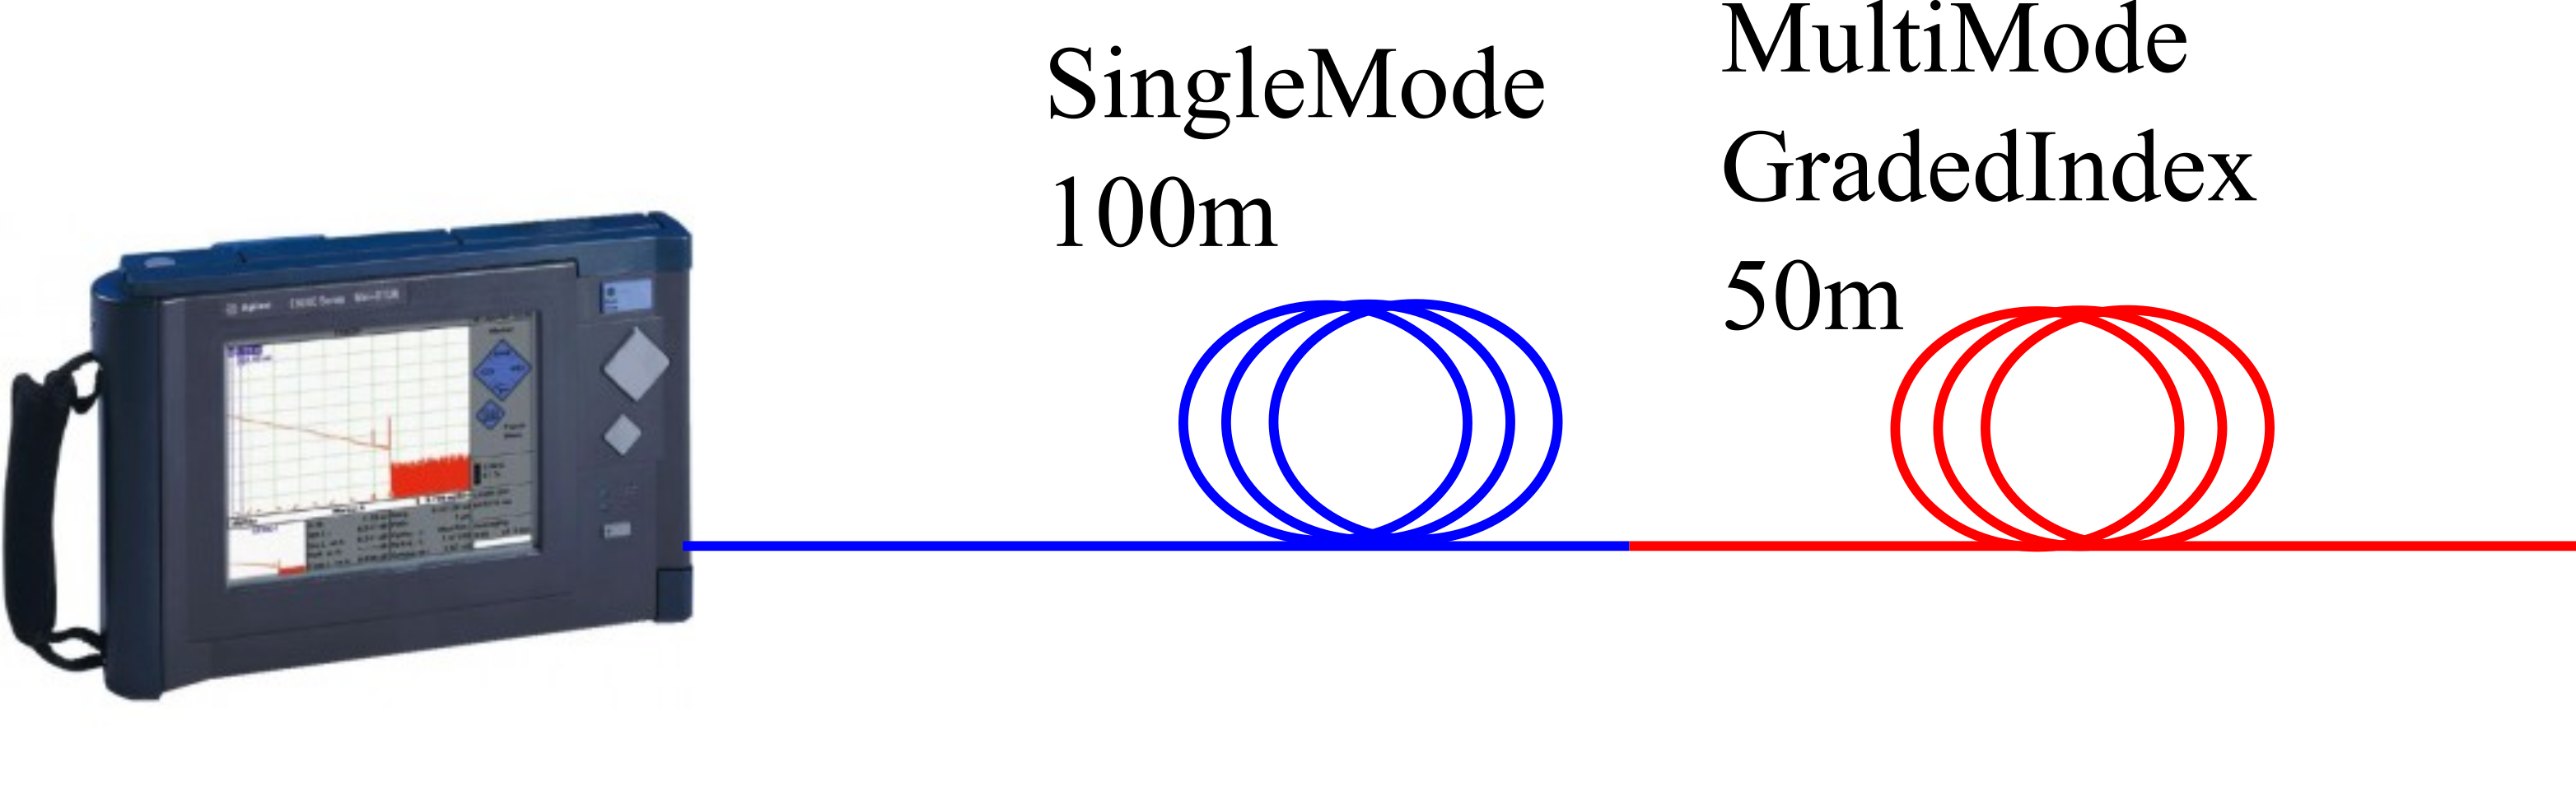
\includegraphics[width=0.6\linewidth]{images/Bab_4/smgi}
			\caption[Trace SMF-SMF]{\small{Rangkaian serat optik SingleMode-MultiModeGradedIndex}}
		\end{figure}
	
		Selanjutnya berikutnya adalah grafik hasil trace OTDR:
		
		\begin{figure}[!ht]
			\centering
			\captionsetup{justification=centering}
			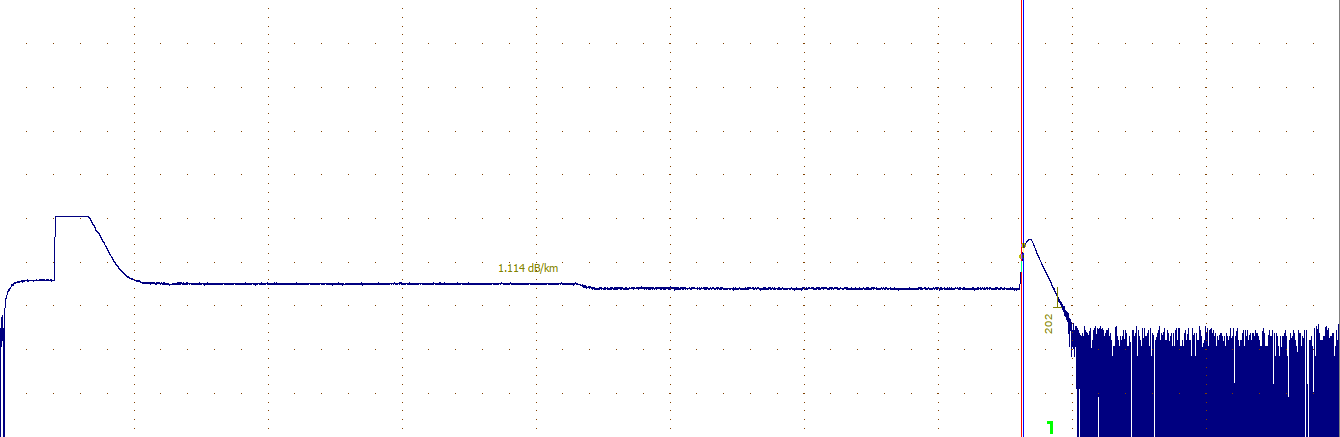
\includegraphics[width=0.9\linewidth]{images/Bab_4/Bab_4_3c1}
			\caption[Trace SM-MMFGI ]{\small{Hasil trace OTDR pada SM-MMFGI normal}}
		\end{figure}
	
		dan berikutnya adalah grafik hasil trace OTDR kondisi dengan gangguan:
		
		\begin{figure}[!ht]
			\centering
			\captionsetup{justification=centering}
			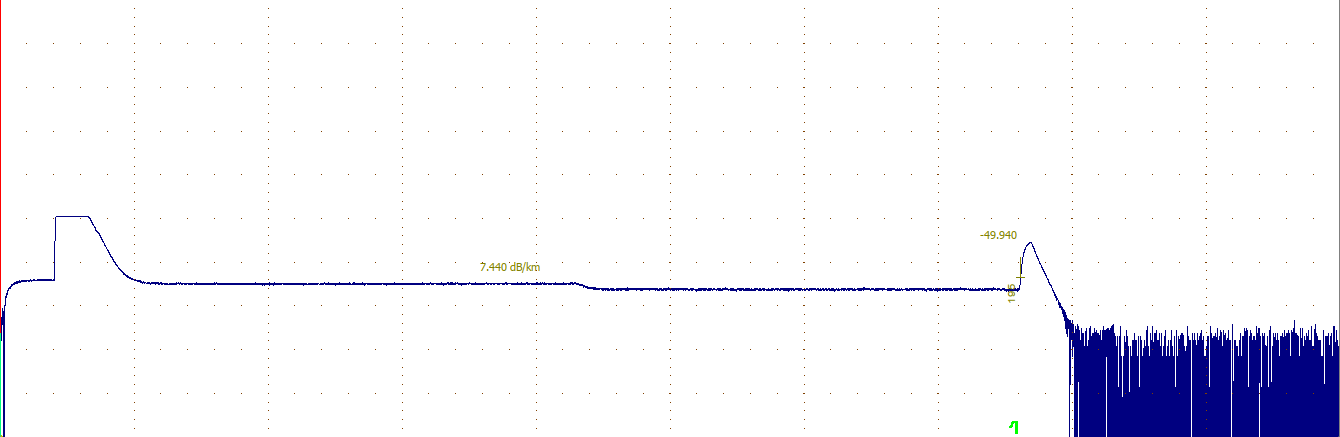
\includegraphics[width=0.9\linewidth]{images/Bab_4/Bab_4_3c2}
			\caption[Trace SM-MMFGI ]{\small{Hasil trace OTDR pada SM-MMFGI dengan gangguan}}
		\end{figure}
	
	    Apabila kedua grafik dibandingkan, maka perubahannya yang dapat terlihat adalah turunnya daya pada event ujung dan splice fiber.
	    Sedangkan pada bagian lainnya didapatkan identik. 
	    Berikut adalah grafiknya (grafik hitam adalah kondisi tanpa gangguan):
	    
	    \begin{figure}[!ht]
	    	\centering
	    	\captionsetup{justification=centering}
	    	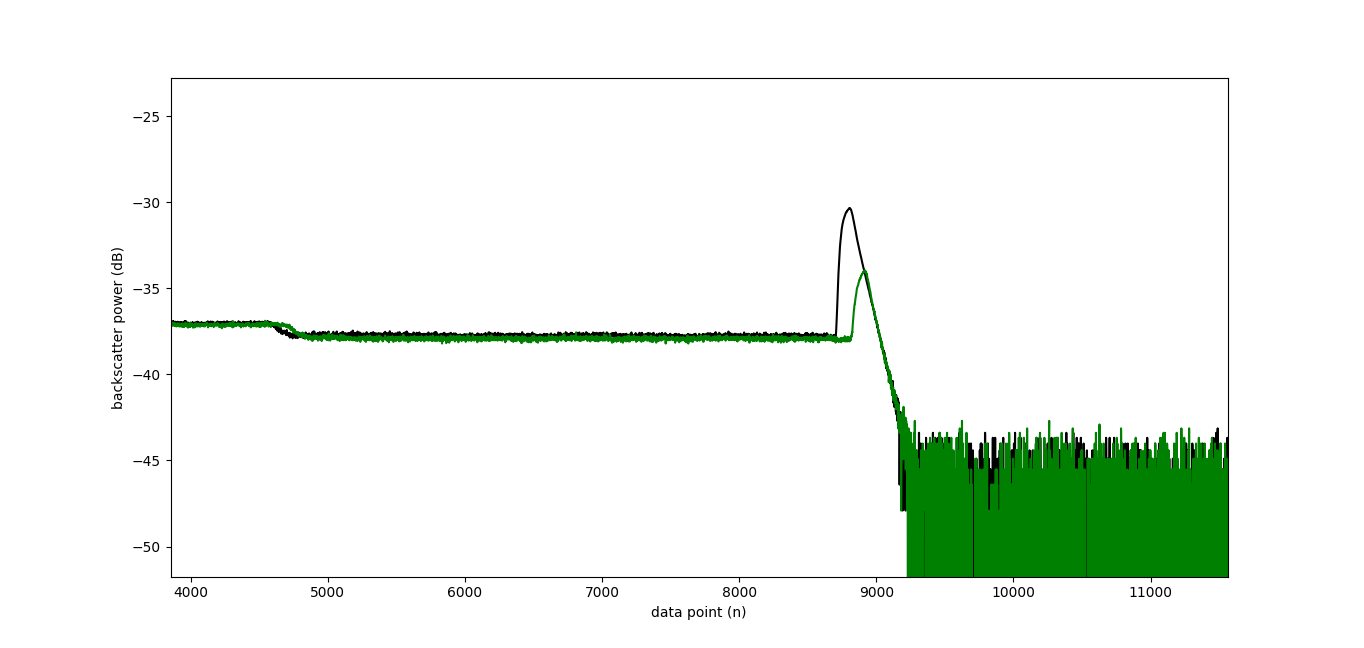
\includegraphics[width=0.8\linewidth]{images/Bab_4/Bab_4_3c3}
	    	\caption[Trace SMF-SMF]{\small{Komparasi kedua grafik pada bagian event ujung fiber}}
	    \end{figure}
	
		
		\item \textbf{Single Mode – Multi Mode Graded Index - Single Mode }
		
		Berikut adalah hasil trace OTDR untuk serat optik SMF dengan tiga splice yaitu antara 1 roll SMF 100m, 1 roll MMF-GI 100m, 1 roll SMF 20 m, dan 10 cm SMF dengan konektor FC (pigtailed)
		Skema rangkaian serat optik (segmen merah adalah yang mendapat gangguan):
		
		\begin{figure}[!ht]
			\centering
			\captionsetup{justification=centering}
			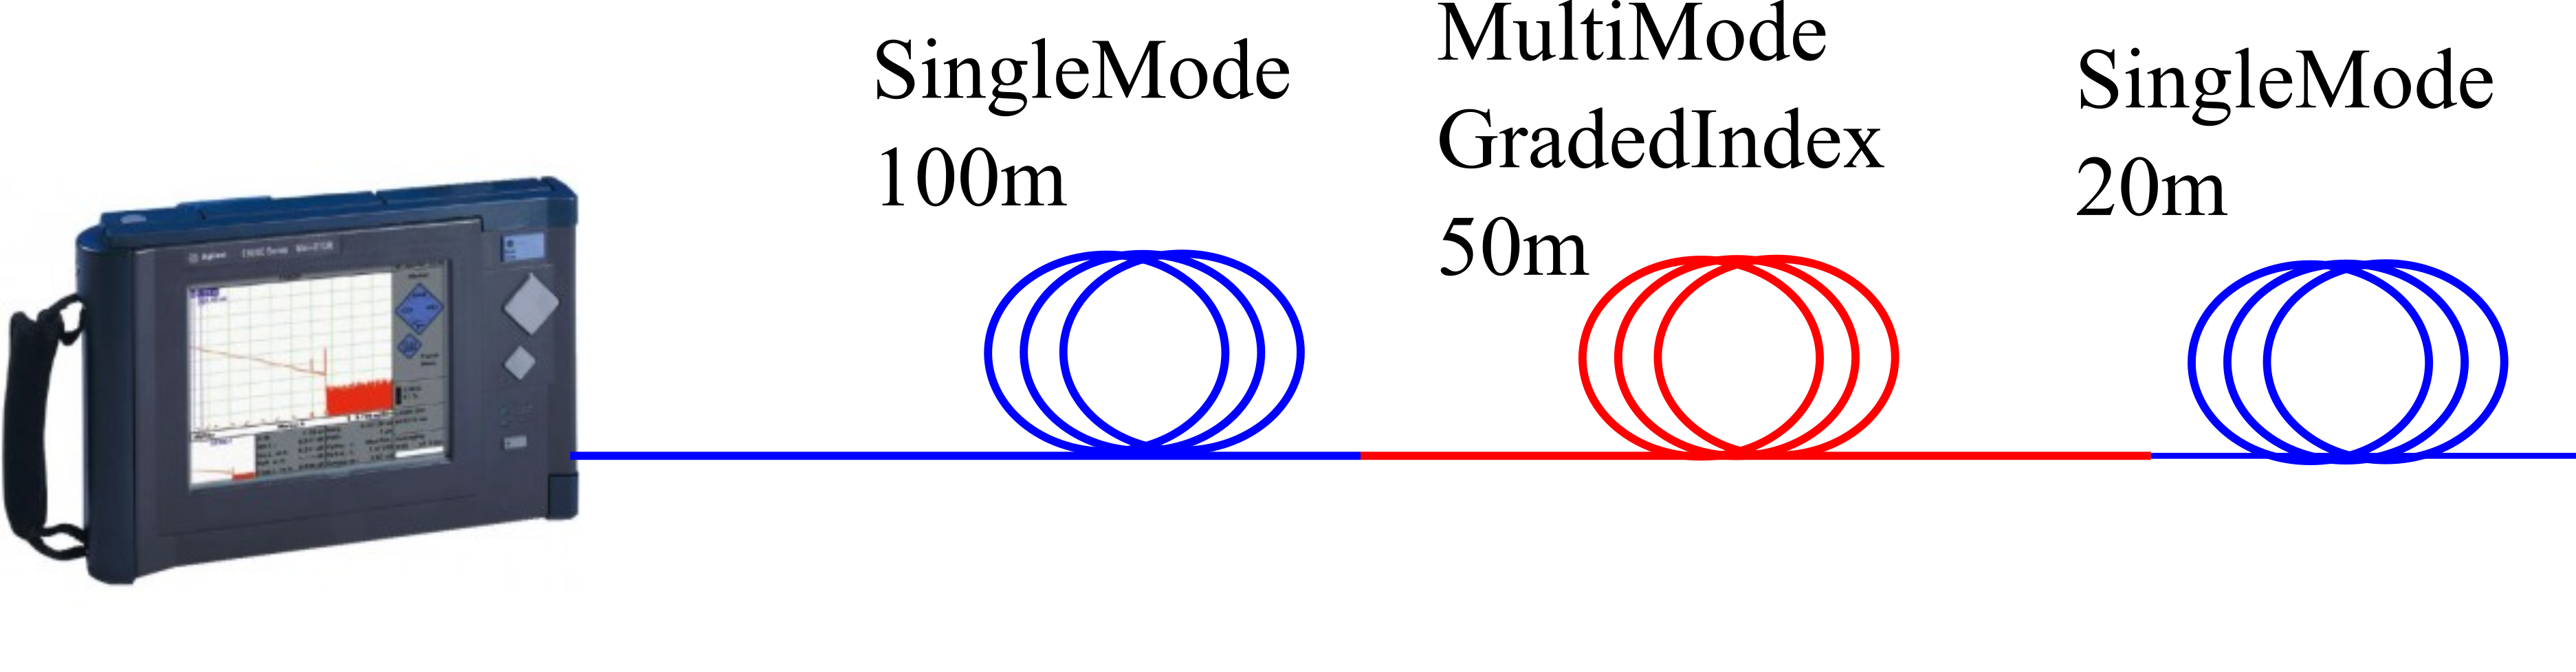
\includegraphics[width=0.5\linewidth]{images/Bab_4/smgism}
			\caption[Trace SMF-SMF]{\small{Rangkaian serat optik SingleMode-MultiModeGradedIndex-SingleMode}}
		\end{figure}
	
		\newpage
		Selanjutnya berikutnya adalah grafik hasil trace OTDR:
		
		\begin{figure}[!ht]
			\centering
			\captionsetup{justification=centering}
			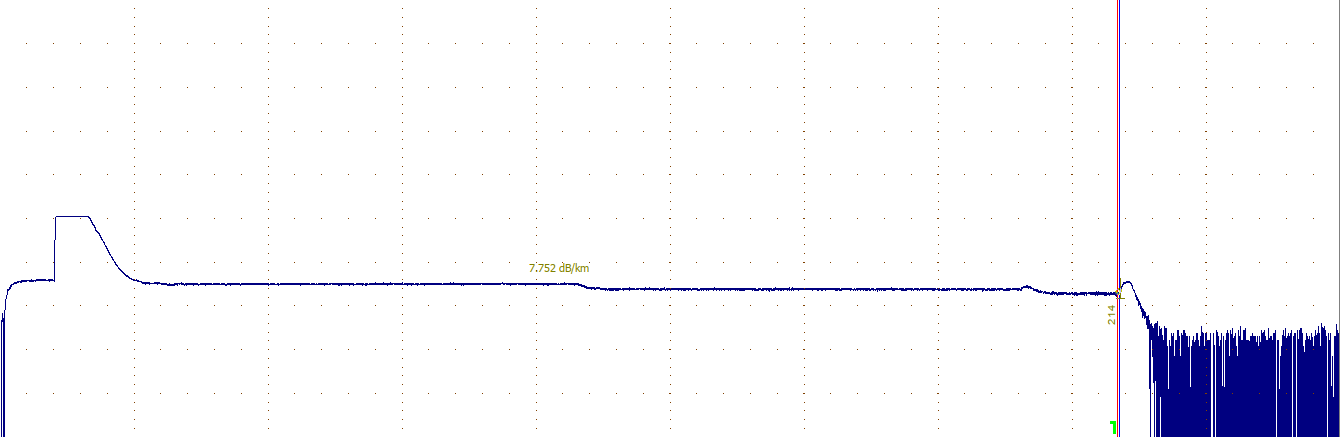
\includegraphics[width=0.8\linewidth]{images/Bab_4/Bab_4_3d1}
			\caption[Trace SM-MMFGI-SM]{\small{Hasil trace OTDR pada SM-MMFGI-SM normal}}
		\end{figure}
	
		dan berikutnya adalah grafik hasil trace OTDR kondisi dengan gangguan:
		
		\begin{figure}[!ht]
			\centering
			\captionsetup{justification=centering}
			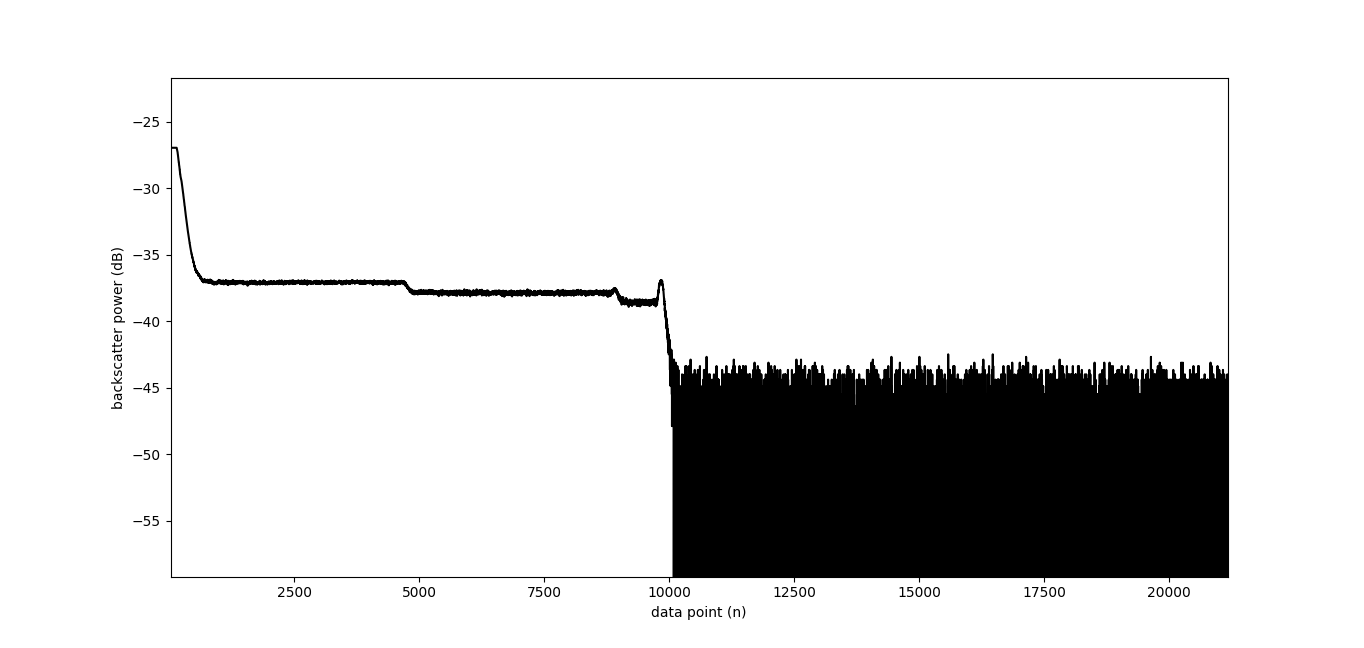
\includegraphics[width=0.8\linewidth]{images/Bab_4/Bab_4_3d2}
			\caption[Trace SM-MMFGI-SM]{\small{Hasil trace OTDR pada SM-MMFGI-SM dengan gangguan}}
		\end{figure}
	
		Apabila kedua grafik dibandingkan, maka perubahannya yang dapat terlihat adalah turunnya daya pada event ujung dan splice fiber.
		Sedangkan pada bagian lainnya didapatkan identik. 
		Berikut adalah grafiknya (grafik hitam adalah kondisi tanpa gangguan):
		
		\begin{figure}[!ht]
			\centering
			\captionsetup{justification=centering}
			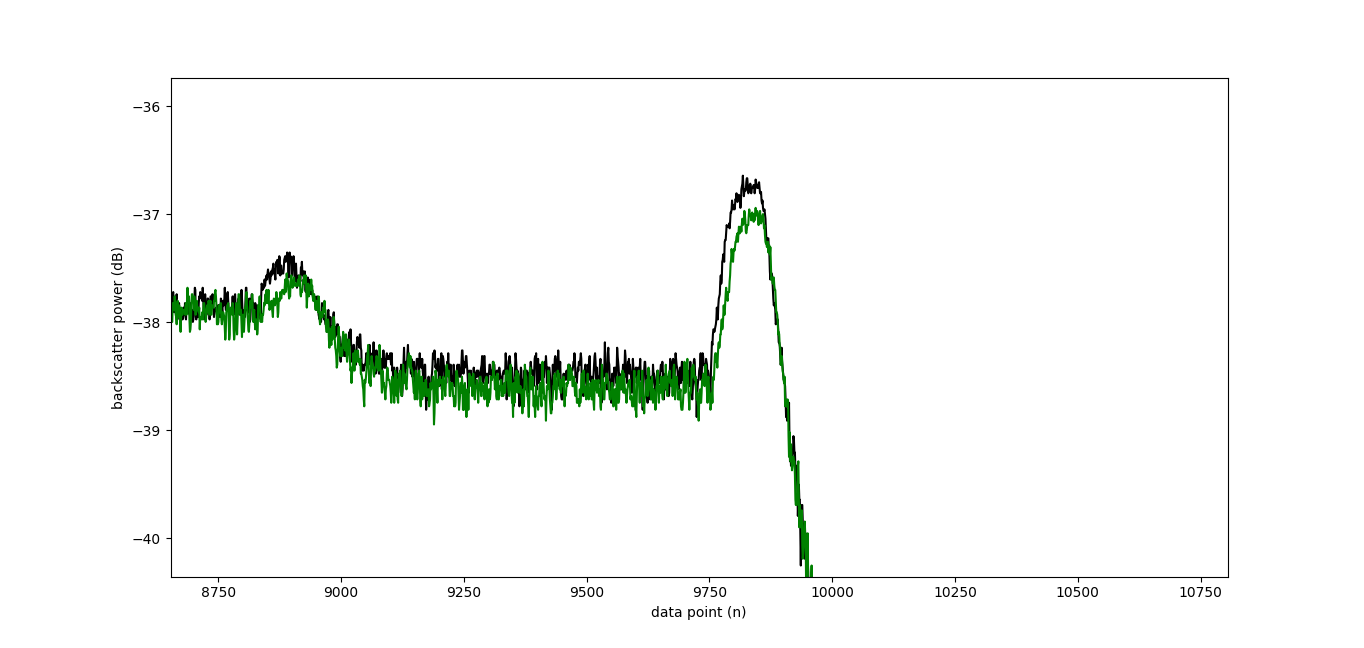
\includegraphics[width=0.8\linewidth]{images/Bab_4/Bab_4_3d3}
			\caption[Trace SMF-SMF]{\small{Komparasi kedua grafik pada bagian event ujung fiber}}
		\end{figure}
		
		\newpage
		\item \textbf{Single Mode – Multi Mode Step Index}
		
		Berikut adalah hasil trace OTDR untuk serat optik SMF dengan tiga splice yaitu antara 1 roll SMF 100m, 1 roll MMF-SI 100m, dan 10 cm SMF dengan konektor FC (pigtailed)
		Skema rangkaian serat optik (segmen merah adalah yang mendapat gangguan):
		
		\begin{figure}[!ht]
			\centering
			\captionsetup{justification=centering}
			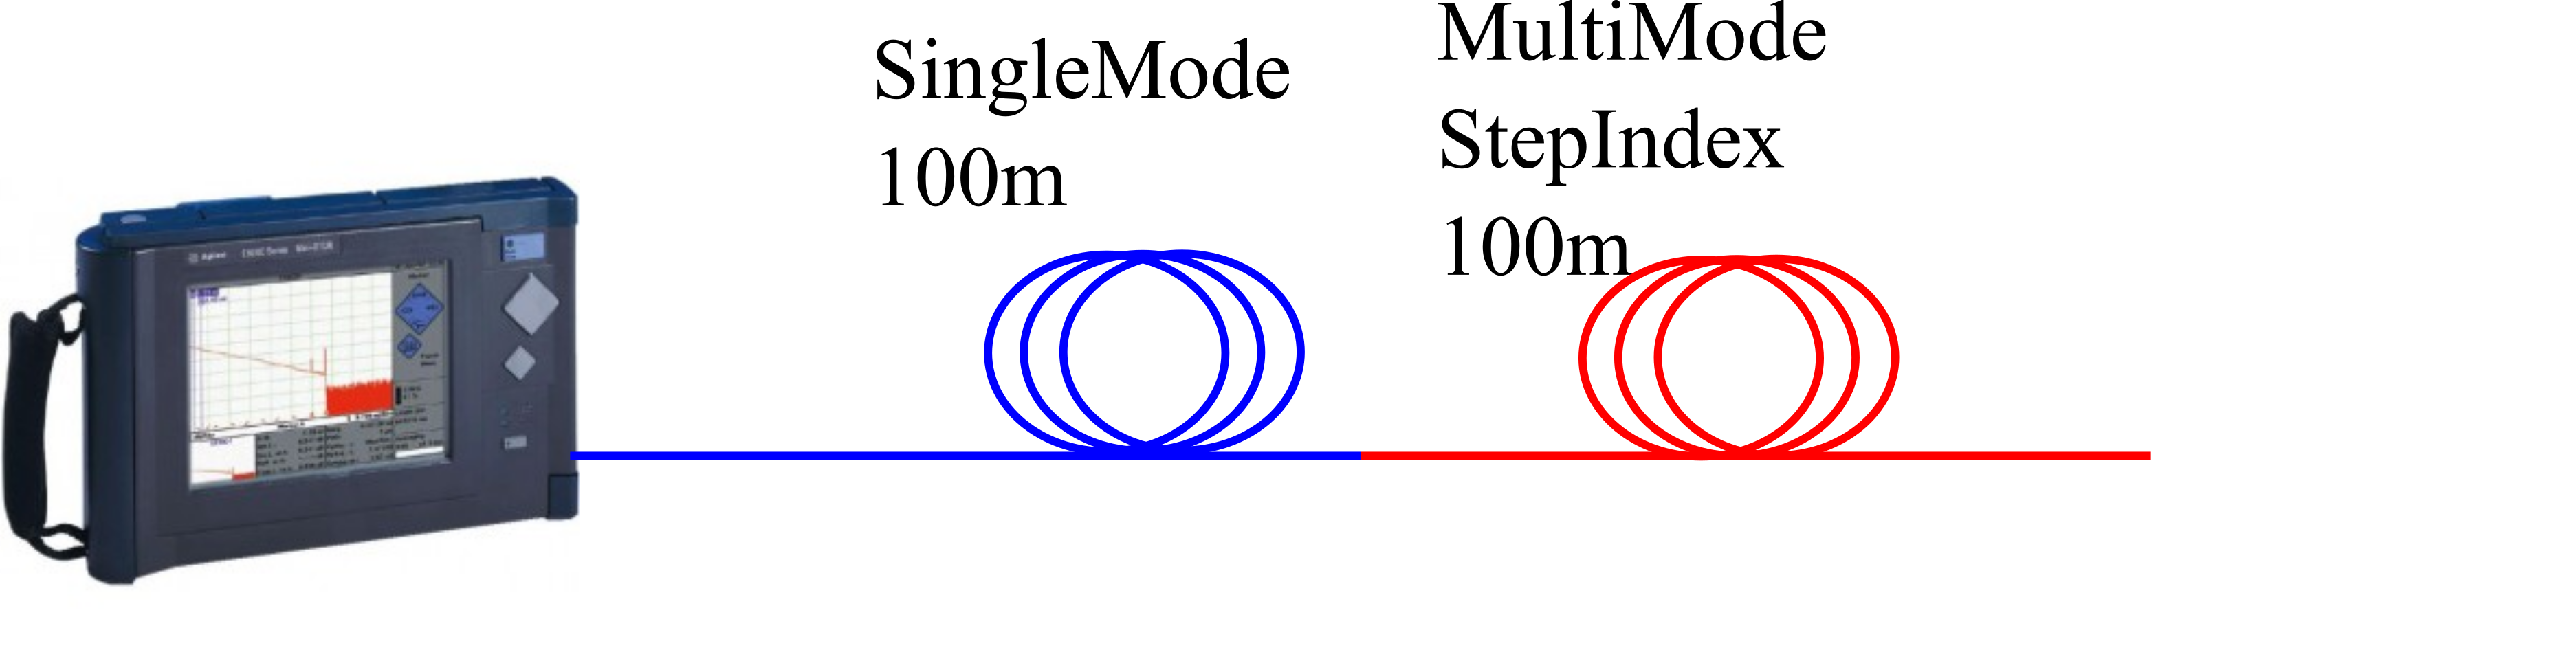
\includegraphics[width=0.7\linewidth]{images/Bab_4/smsi}
			\caption[Trace SMF-SMF]{\small{Rangkaian serat optik SingleMode-MultiModeStepIndex}}
		\end{figure}
	
		Hasil trace pada rangkaian serat optik ini didapat tidak merespon gangguan yang dikenakan pada segmen MultiModeStepIndex.
		Sehingga grafik trace tidak memiliki perbedaan antara tanpa dan dengan adanya gangguan.
		
		\begin{figure}[!ht]
			\centering
			\captionsetup{justification=centering}
			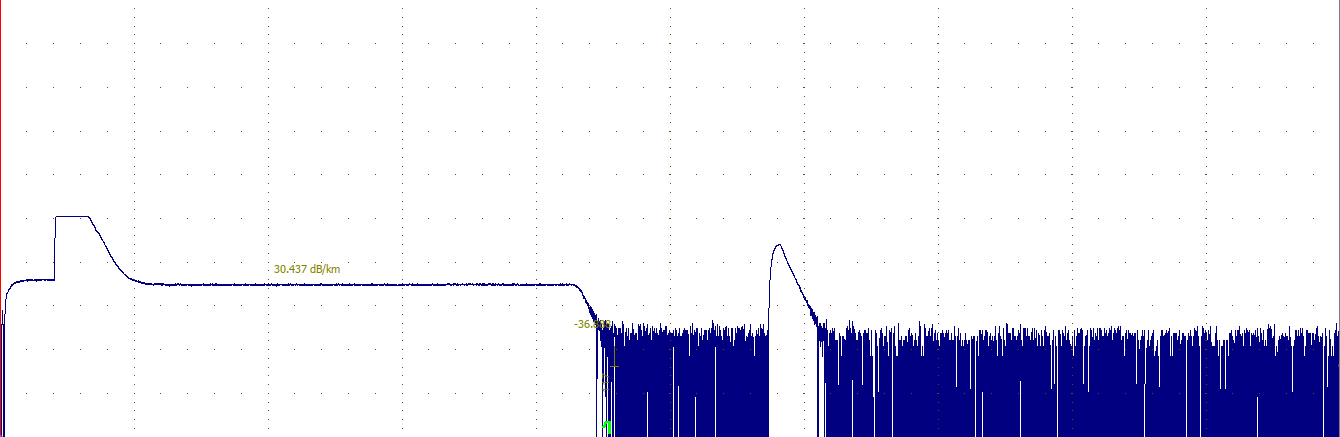
\includegraphics[width=\linewidth]{images/Bab_4/Bab_4_3e1}
			\caption[Trace SM-MMFSI]{\small{Hasil trace OTDR pada baik SM-MMFSI normal maupun SM- MMFSI dengan gangguan}}
		\end{figure}
	
%=============================================================================
\newpage	
	
		\item \textbf{Single Mode – Multi Mode Step Index- Single Mode }
		
		Berikut adalah hasil trace OTDR untuk serat optik SMF dengan tiga splice yaitu antara 1 roll SMF 100m, 1 roll MMF-SI 50m, 1 roll SMF 20 m, dan 10 cm SMF dengan konektor FC (pigtailed).
		Skema rangkaian serat optik (segmen merah adalah yang mendapat gangguan):
		
		\begin{figure}[!ht]
			\centering
			\captionsetup{justification=centering}
			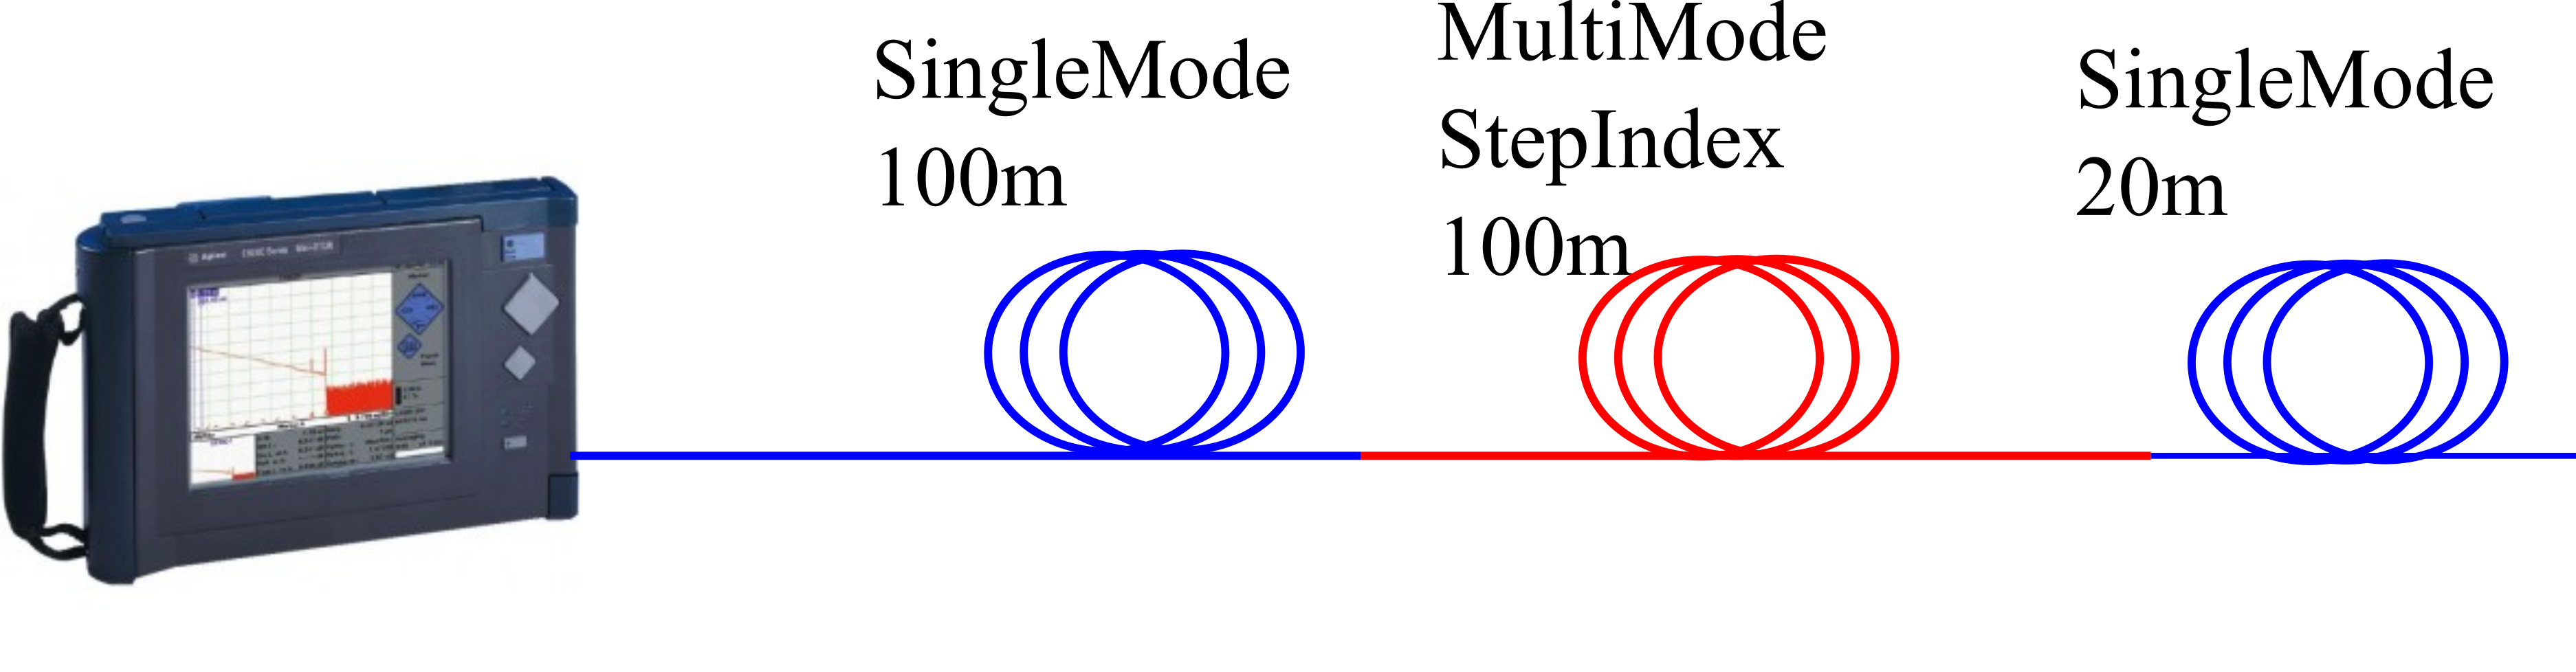
\includegraphics[width=0.7\linewidth]{images/Bab_4/smsism}
			\caption[Trace SMF-SMF]{\small{Rangkaian serat optik SingleMode-MultiModeStepIndex-SingleMode}}
		\end{figure}
	
		Hasil trace pada rangkaian serat optik ini didapat tidak merespon gangguan yang dikenakan pada segmen MultiModeStepIndex.
		Sehingga grafik trace tidak memiliki perbedaan antara tanpa dan dengan adanya gangguan.
		
		\begin{figure}[!ht]
			\centering
			\captionsetup{justification=centering}
			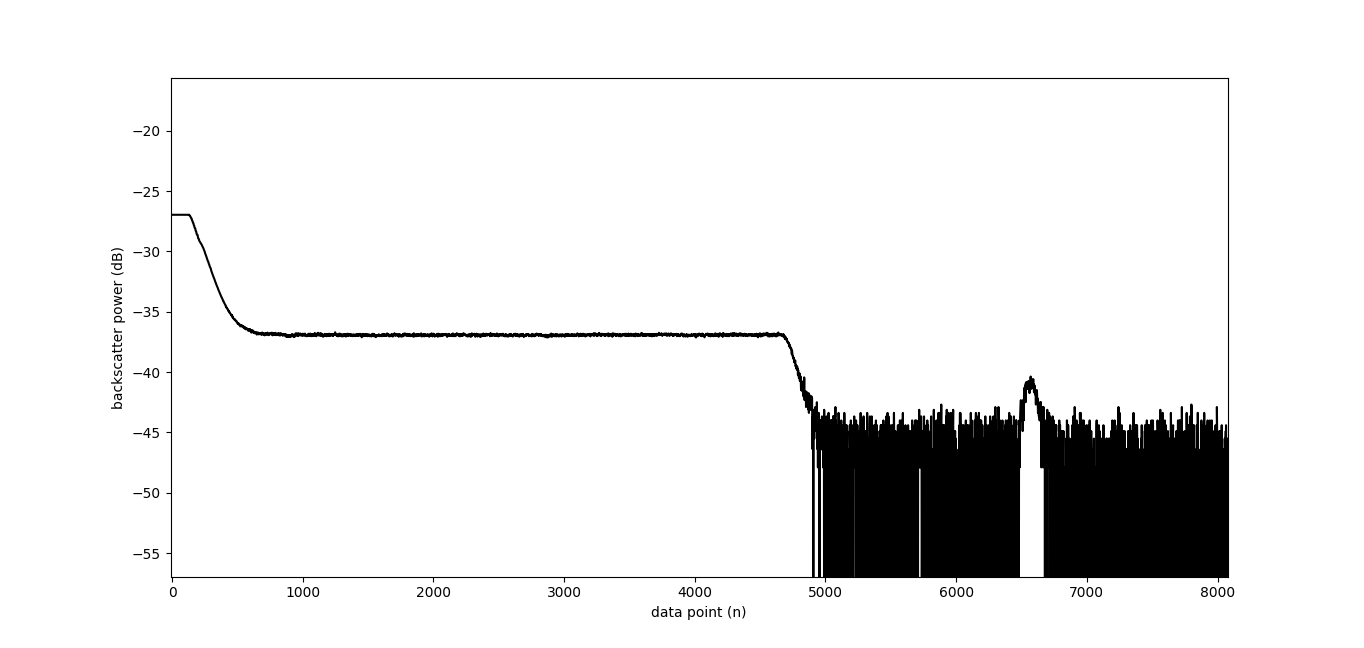
\includegraphics[width=\linewidth]{images/Bab_4/Bab_4_3f1}
			\caption[Trace SM-MMFSI-SM ]{\small{Hasil trace OTDR pada baik SM-MMFSI-SM  normal maupun SM-MMFSI-SM  dengan gangguan}}
		\end{figure}
	
	\end{enumerate}
	
%============================================================================
		
	\newpage
	
	\subsection{Hasil uji Displacement}
	Dengan memperhatikan hasil-hasil sebelumnya, maka dilakukan uji displacement dengan menggunakan:
	\begin{itemize}
		\item Konfigurasi serat optik SingleMode-MultiModeGradedIndex-SingleMode
		\item Lebar pulsa adalah 10 ns dan selang averaging adalah 45 ms
	\end{itemize}

	Skema untuk pengujian dengan MultiModeGradedIndex 1 meter adalah:
	
	\begin{figure}[!ht]
		\centering
		\captionsetup{justification=centering}
		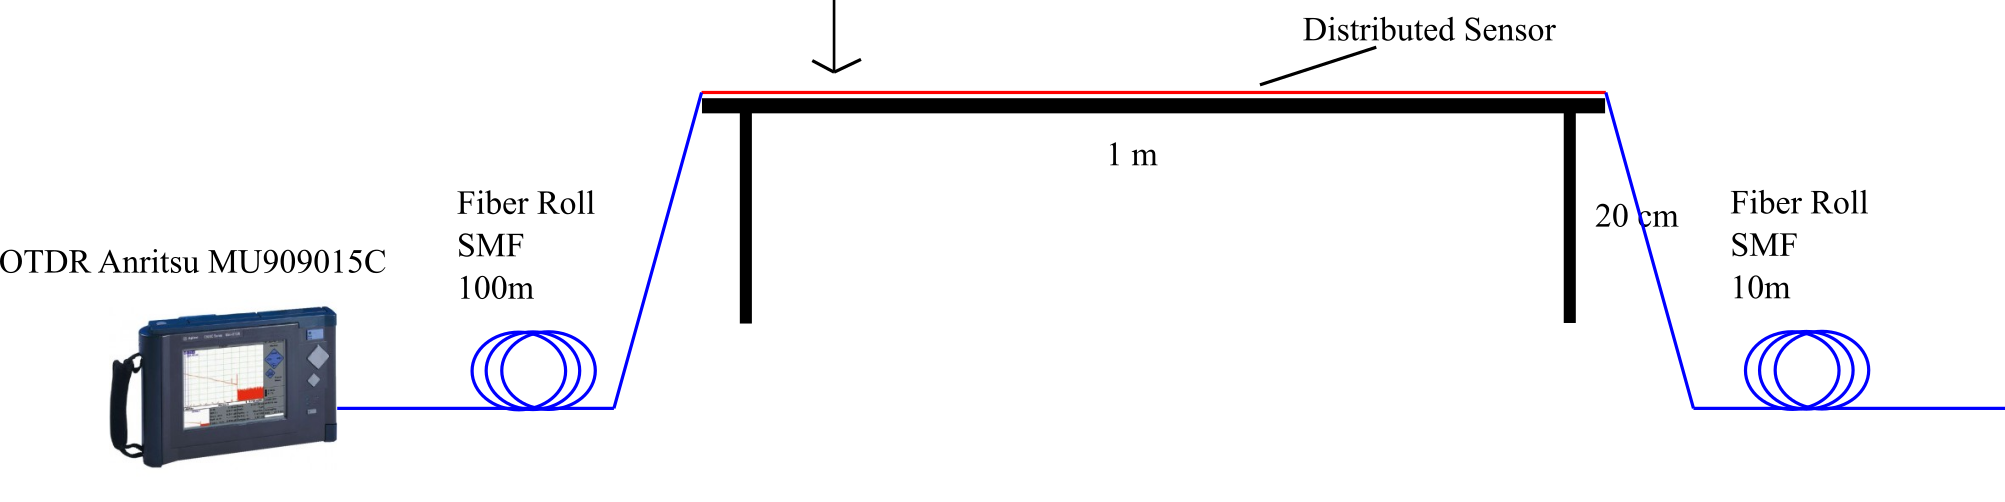
\includegraphics[width=0.7\linewidth]{images/Bab_4/uji_1m}
		\caption[Trace SMF-SMF]{\small{Skema uji SingleMode-MultiModeGradedIndex-SingleMode 1m}}
	\end{figure}
	
	Grafik hasil trace secara umum di semua pengujian 1 meter adalah sebagai berikut:
	
	\begin{figure}[!ht]
		\centering
		\captionsetup{justification=centering}
		\begin{subfigure}[h]{0.8\textwidth}
			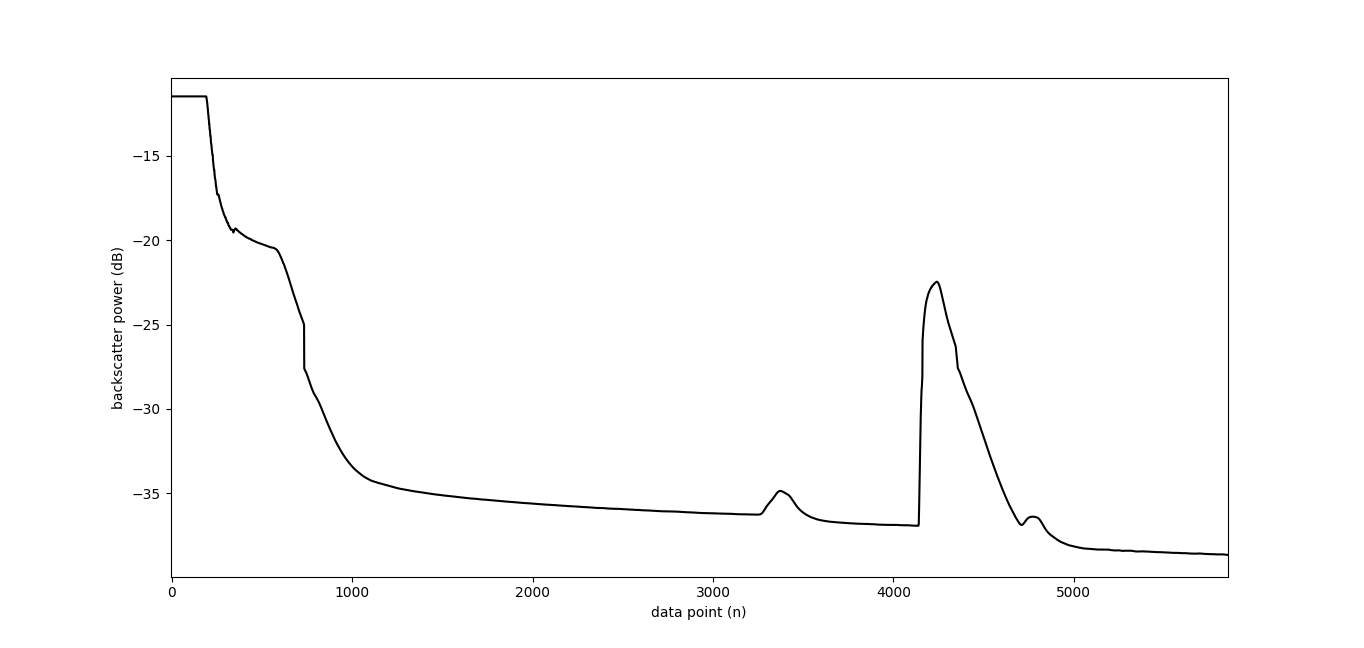
\includegraphics[width=\textwidth]{images/Bab_4/Bab_4_5d1}	
			\caption{\small{Grafik trace dasar}}		
		\end{subfigure}
		\begin{subfigure}[h]{0.8\textwidth}
			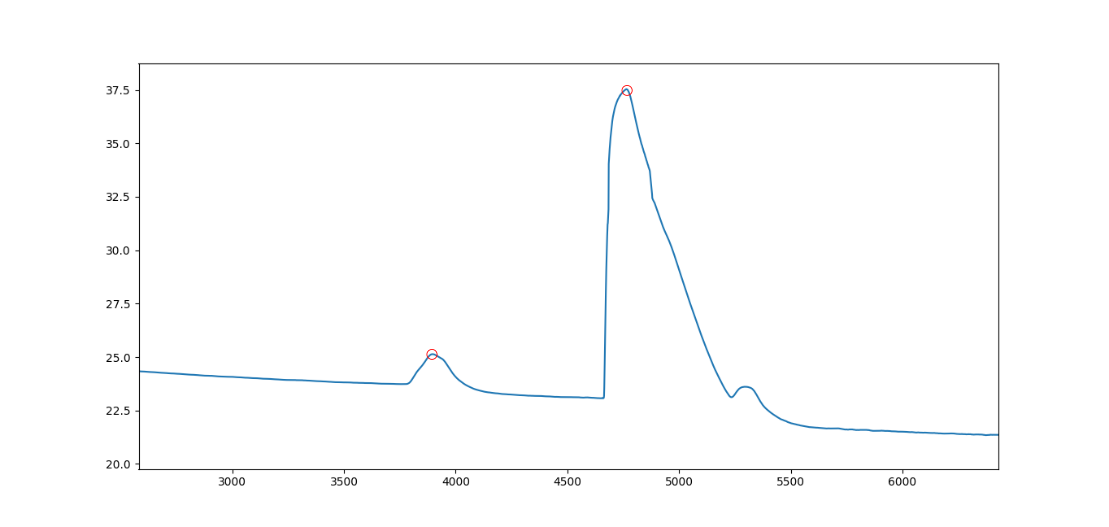
\includegraphics[width=\linewidth]{images/Bab_4/Bab_4_5d2}
			\caption{\small{Nilai puncak event fiber \textit{Splice} dan \textit{End}}}			
		\end{subfigure}
		\caption[Uji Pagar]{\small{Grafik hasil Trace untuk panjang 1 meter}}
	\end{figure}

	Selanjutnya skema untuk pengujian dengan MultiModeGradedIndex 5 meter adalah:
	
	\begin{figure}[!ht]
		\centering
		\captionsetup{justification=centering}
		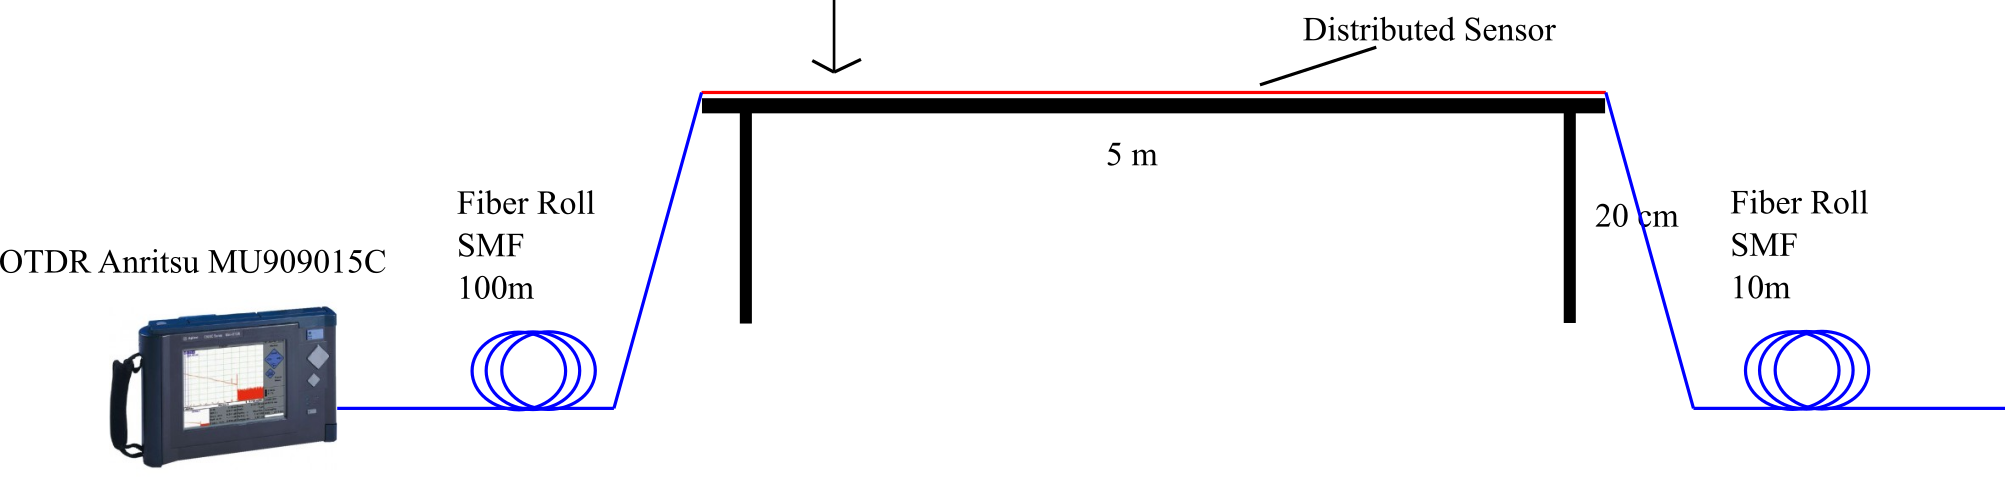
\includegraphics[width=0.7\linewidth]{images/Bab_4/uji_5m}
		\caption[Trace SMF-SMF]{\small{Skema uji SingleMode-MultiModeGradedIndex-SingleMode 1m}}
	\end{figure}
	
	dan grafik hasil trace secara umum di semua pengujian 5 meter adalah sebagai berikut:
	
	\begin{figure}[!ht]
		\centering
		\captionsetup{justification=centering}
		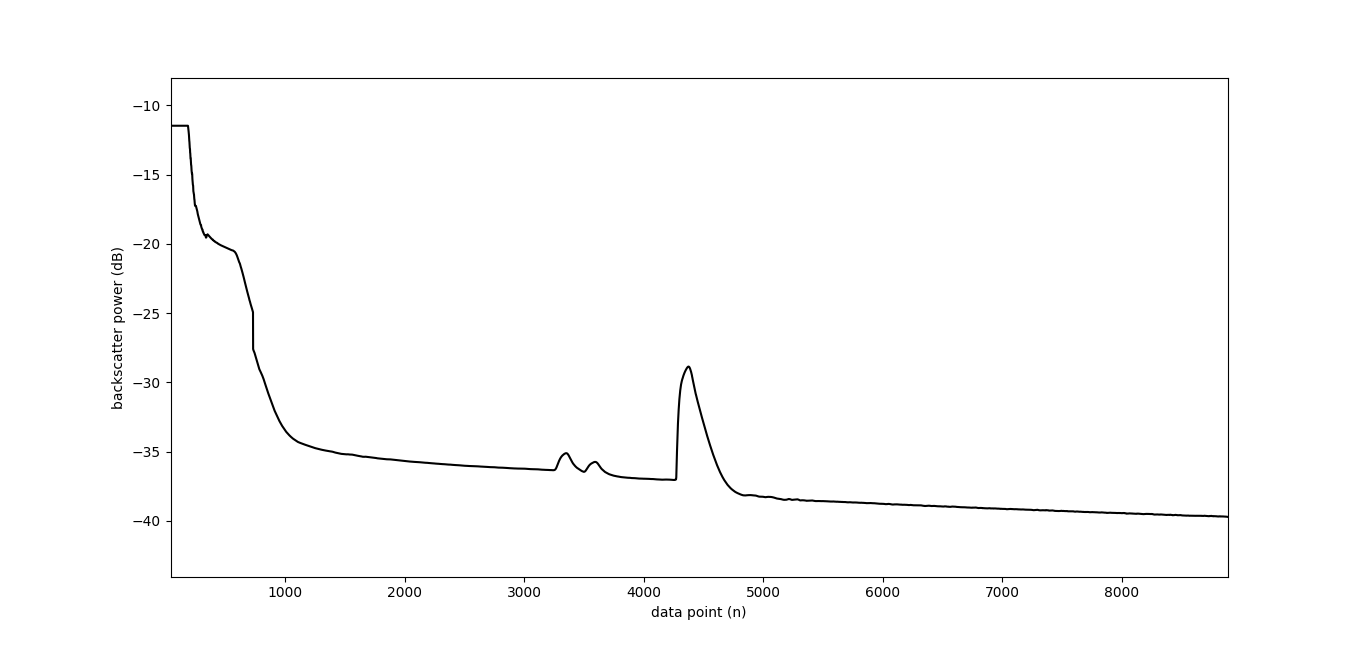
\includegraphics[width=\textwidth]{images/Bab_4/Bab_4_5e1}	
		\caption{\small{(a) Grafik trace dasar}}
	\end{figure}
	
	\newpage
	\begin{figure}[!ht]
		\centering
		\captionsetup{justification=centering}
		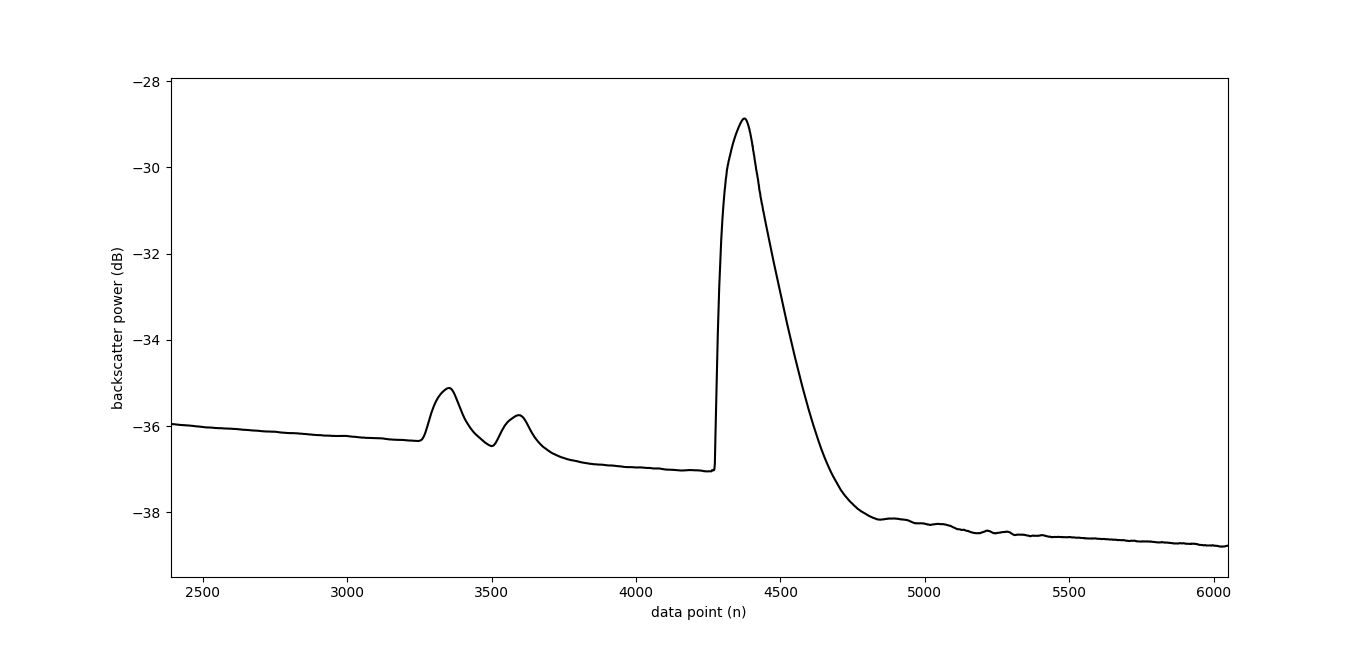
\includegraphics[width=\textwidth]{images/Bab_4/Bab_4_5e2}	
		\caption{\small{(b) Nilai puncak event fiber \textit{Splice} dan \textit{End}}}
	\end{figure}
	
	\newpage
	Terakhir skema untuk pengujian dengan MultiModeGradedIndex 1 meter dengan 2 segmen adalah:
	
	\begin{figure}[!ht]
		\centering
		\captionsetup{justification=centering}
		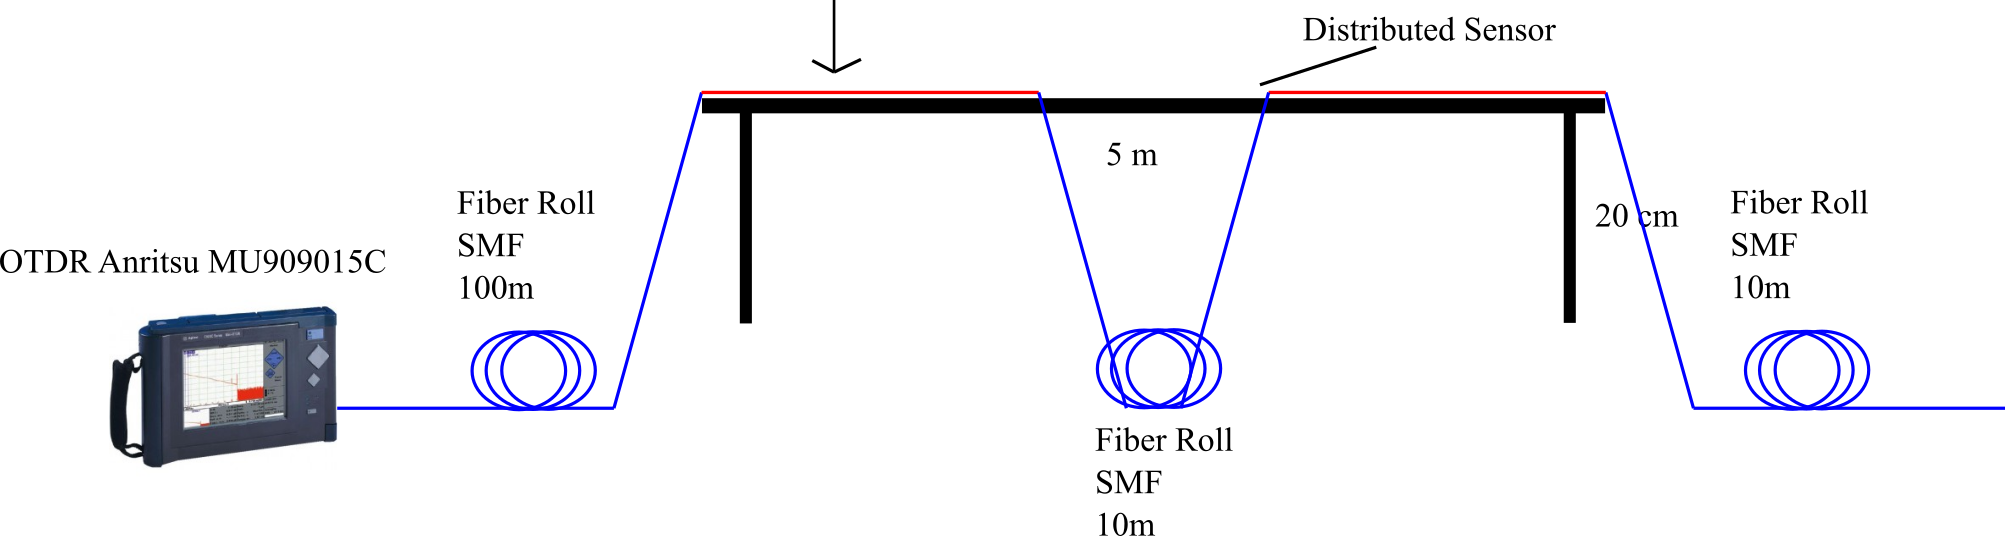
\includegraphics[width=0.7\linewidth]{images/Bab_4/uji2_1m}
		\caption[Trace SMF-SMF]{\small{Skema uji SingleMode-MultiModeGradedIndex-SingleMode 1m}}
	\end{figure}
	
	Selanjutnya, didapatkan selisih semua nilai puncak event terhadap kondisi tanpa gangguan,
	sehingga dapat ditemukan respon fiber di setiap posisi dan ukuran \textit{displacement}.
	
	\begin{align}
		\Delta P = abs(max(E_1) - max(E_0))
	\end{align}
	
	Dengan $E_1$ adalah event tertentu pada kondisi ada gangguan dan $E_0$ event tertentu pada kondisi tanpa gangguan.
	
	Berikut adalah grafik respon pada event \textit{splice} dan \textit{end}.
	
	\begin{figure}[!ht]
		\centering
		\captionsetup{justification=centering}
		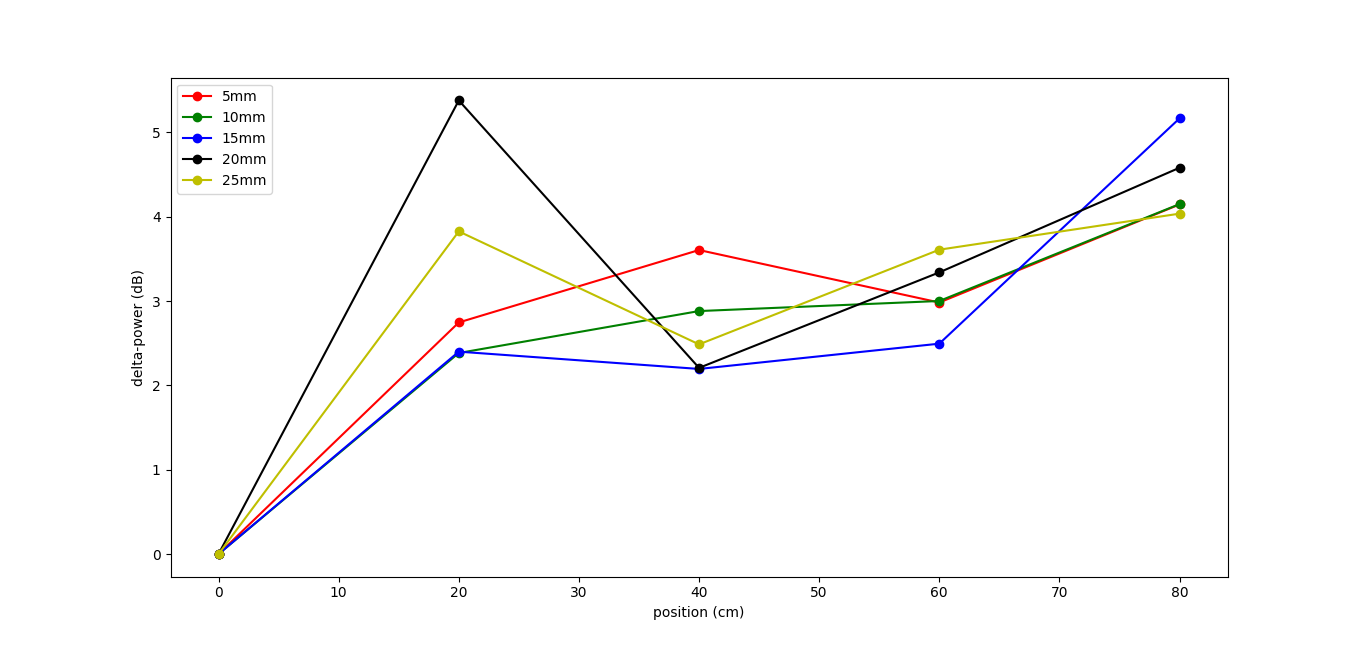
\includegraphics[width=0.9\textwidth]{images/Bab_4/Bab_4_5f1}	
		\caption{\small{(a) Respon fiber end}}
	\end{figure}
	
	\begin{figure}[!ht]
		\centering
		\captionsetup{justification=centering}
		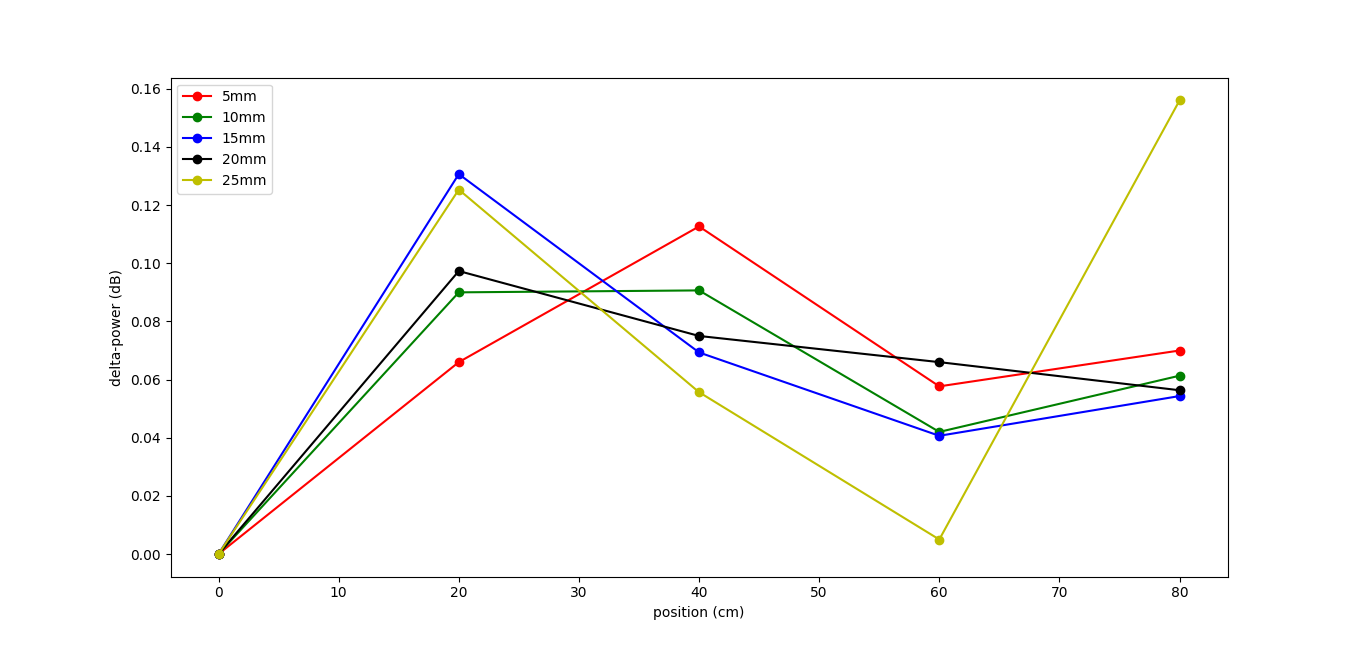
\includegraphics[width=0.9\textwidth]{images/Bab_4/Bab_4_5f2}	
		\caption{\small{(b) Respon fiber splice}}
	\end{figure}

	\newpage
	Dapat terlihat bahwa respon puncak event fiber-end adalah gradien positif terhadap posisi displacement.
	
	Sedangkan untuk event fiber-splice tidak memberikan respon signifikan terhadap jarak.

	Selanjutnya untuk grafik 5 meter adalah sebagai berikut:
	
	\begin{figure}[!ht]
		\centering
		\captionsetup{justification=centering}
		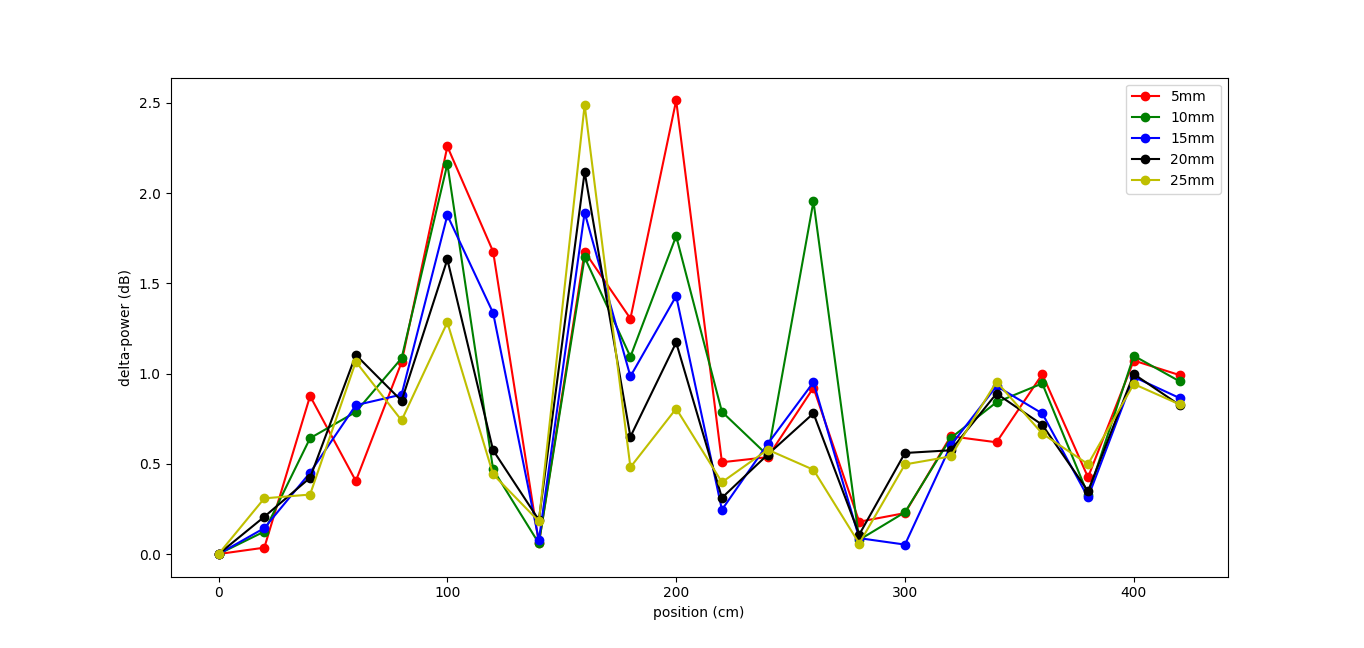
\includegraphics[width=0.9\textwidth]{images/Bab_4/Bab_4_5g1}	
		\caption{\small{(a) Respon fiber end}}
	\end{figure}
	
	\begin{figure}[!ht]
		\centering
		\captionsetup{justification=centering}
		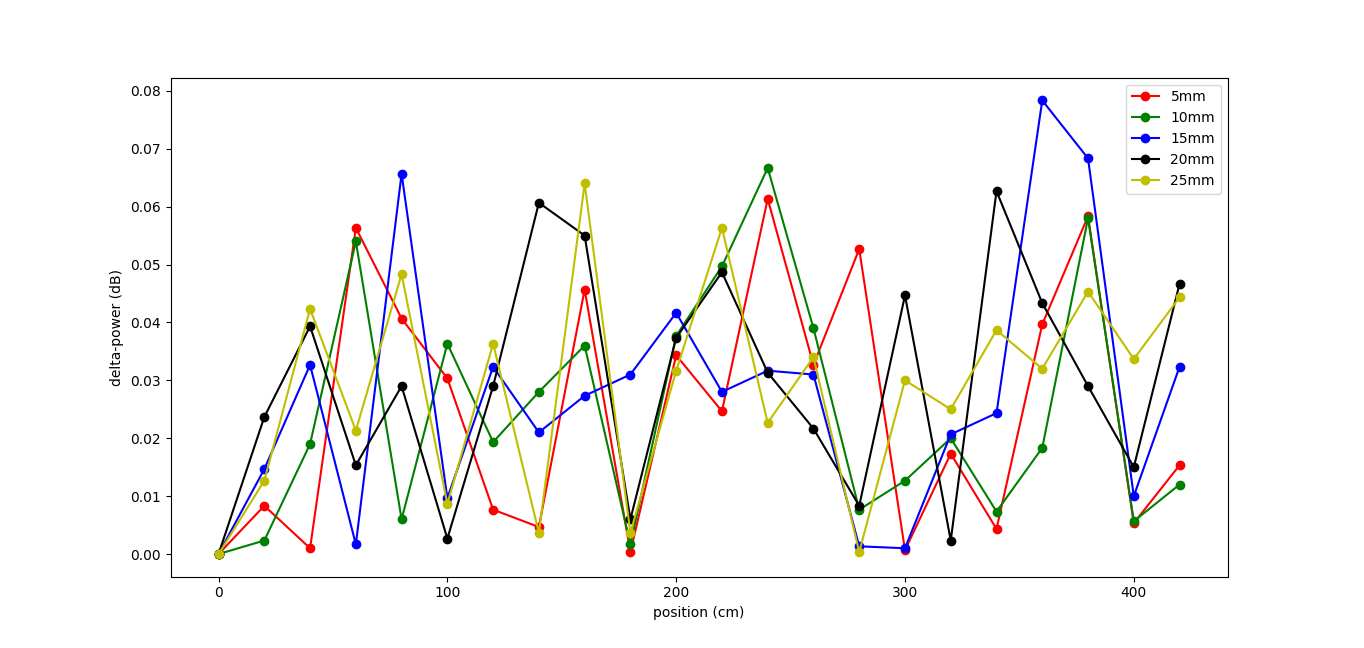
\includegraphics[width=0.8\textwidth]{images/Bab_4/Bab_4_5g2}	
		\caption{\small{(b) Respon fiber splice}}
	\end{figure}

	Dapat terlihat untuk panjang fiber 5 meter, fiber-end memiliki respon terhadap posisi displacement, namun bukan berupa gradien positif. 
	Sedangkan untuk event fiber-splice tidak menunjukkan respon yang memiliki arti sebagaimana pada event splice pada panjang 1 meter.
	
	Selanjutnya uji untuk 2 segmen multimode, hasil grafiknya:
	
	\begin{figure}[!ht]
		\centering
		\captionsetup{justification=centering}
		\begin{subfigure}[h]{0.9\textwidth}
			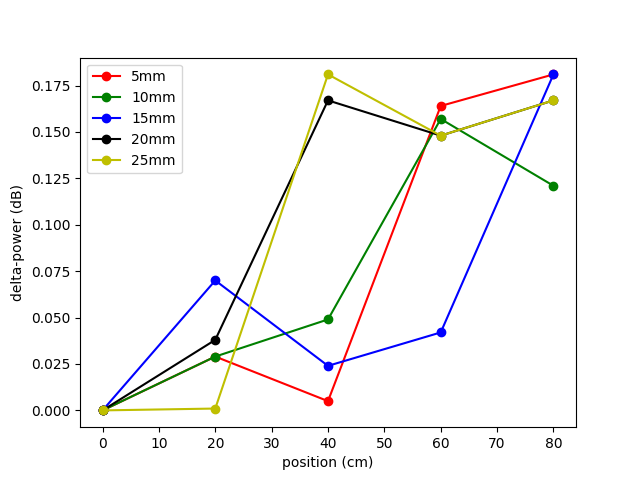
\includegraphics[width=\textwidth]{images/Bab_4/fiber_A_end}	
			\caption{\small{Respon Fiber End pada segmen pertama}}		
		\end{subfigure}
		\begin{subfigure}[h]{0.9\textwidth}
			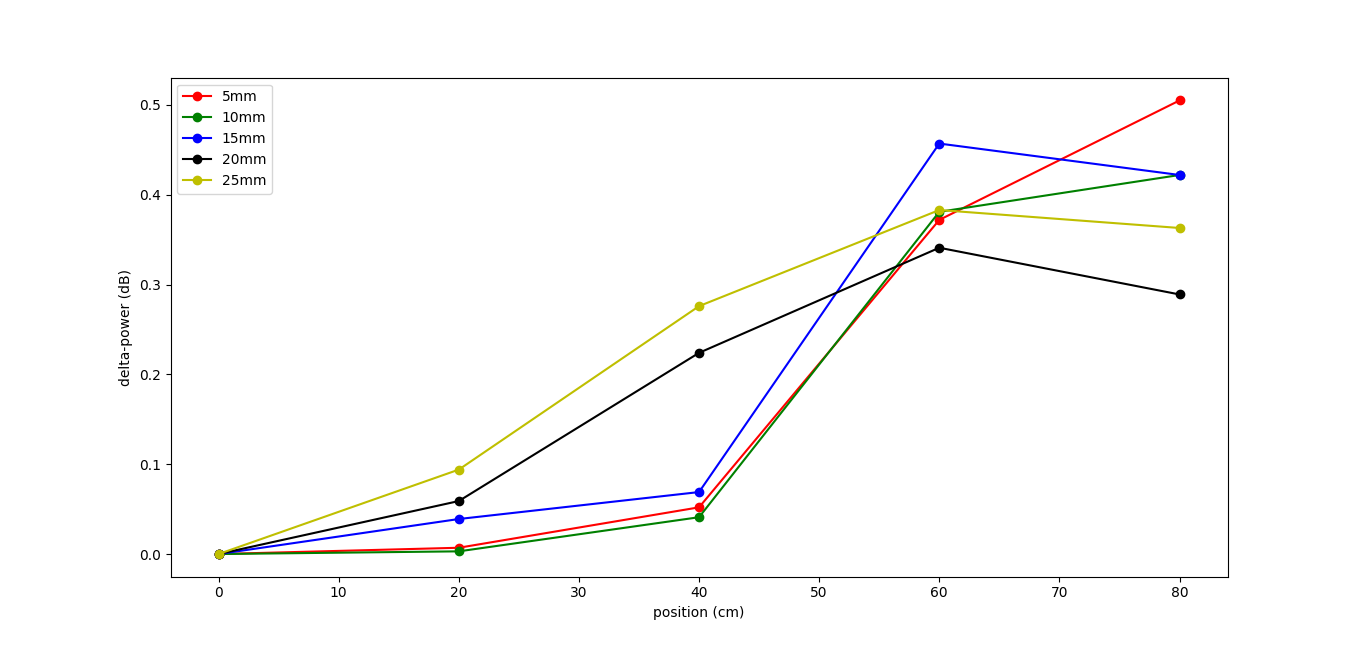
\includegraphics[width=\linewidth]{images/Bab_4/fiber_B_end}
			\caption{\small{Respon Fiber End pada segmen kedua}}			
		\end{subfigure}
		\caption[belum ada judul]{\small{Respon Fiber End pada setiap segmen}}
	\end{figure}

	Dapat terlihat bahwa respon puncak event fiber-end adalah gradien positif terhadap posisi displacement.
	Perbedaan antara segmen pertama dan kedua ada pada rentang $\Delta P$ yang dihasilkan dimana segmen kedua lebih besar.

\newpage
	\subsection{Pendekatan Model}
	
	Dengan memperhatikan hasil pada 1 meter, apabila diambil nilai posisi sebagai input sedangkan selisih power \textit{backscatter} sebagai ouput.
	Maka kemudian dapat dicari pendekatan model yaitu semisal dengan regresi linear akan mendapatkan grafik respon.
	Berikut grafik dan persamaan pendekatan untuk 1 meter:
	
	\begin{figure}[!ht]
		\centering
		\captionsetup{justification=centering}
		\begin{subfigure}[h]{\textwidth}
			\includegraphics[width=\textwidth]{images/Bab_4/lingres_fend}	
			\caption{\small{Pendekatan Respon Fiber End pada segmen pertama}}		
		\end{subfigure}
		\begin{subfigure}[h]{\textwidth}
			\includegraphics[width=\linewidth]{images/Bab_4/lingres_fspi}
			\caption{\small{Pendekatan Respon Fiber End pada segmen kedua}}			
		\end{subfigure}
		\caption[belum ada judul]{\small{Pendekatan Respon Fiber End pada setiap segmen}}
	\end{figure}
	

%=============================================================================

\newpage
\thispagestyle{empty}
\mbox{}

%=============================================================================
% Kesimpulan

\newpage
\section{Kesimpulan}

\begin{center}
	{\large \textbf{BAB V}} \\
	{\large \textbf{Kesimpulan dan Saran}}
\end{center}

\subsection{Kesimpulan}

Berikut adalah kesimpulan untuk menjawab rumusan masalah:

\begin{itemize}
	\item Gangguan mekanis (\textit{Peturbation}) dapat dideteksi dengan instrumen OTDR berdasarkan respon nilai refleksi pada event \textit{fiber end}.
	\item Dengan mendapatkan selisih nilai maksimum pada event \textit{fiber end} saat ada gangguan dan tidak ada gangguan, dapat diperkirakan posisi displacement.
	\item Konfigurasi serat optik yang dapat diusulkan adalah SingleMode-MultiModeGraded-SingleMode dengan panjang segmen Multimode adalah 1m.
\end{itemize}
	
\subsection{Saran}

%=============================================================================

\newpage
\thispagestyle{empty}
\mbox{}

%=============================================================================
% Daftar Pustaka
\newpage
	\section{Daftar Pustaka}
	
	\begin{center}
		\textbf{Daftar Pustaka}
	\end{center}
	
	\bibliographystyle{IEEEtran}
	\bibliography{/home/achmadi/Documents/BibTex/library.bib}
%	%\bibliography{/home/fotoniks/Mendeley_BibTex/library.bib}
	
\end{document}
